\documentclass[a4paper,12pt]{article}

\usepackage[utf8]{inputenc}
\usepackage{polski}
\usepackage[polish]{babel}
\usepackage{graphicx}
\usepackage{url}
\usepackage{amsfonts}
\usepackage{amsmath}
\usepackage{float}
\usepackage{subfig}

%%
%% pygments.tex
%%
%% Made by Jakub Kuźma
%% Login   <kuba@ibm>
%%
%% Started on  Sat Oct 25 02:13:17 2008 Jakub Kuźma
%% Last update Sat Oct 25 02:13:17 2008 Jakub Kuźma
%%

\usepackage{fancyvrb}
\usepackage{color}

\newcommand\at{@}
\newcommand\lb{[}
\newcommand\rb{]}
\newcommand\PYbg[1]{\textcolor[rgb]{0.00,0.50,0.00}{\textbf{#1}}}
\newcommand\PYbf[1]{\textcolor[rgb]{0.73,0.40,0.53}{\textbf{#1}}}
\newcommand\PYbe[1]{\textcolor[rgb]{0.40,0.40,0.40}{#1}}
\newcommand\PYbd[1]{\textcolor[rgb]{0.73,0.13,0.13}{#1}}
\newcommand\PYbc[1]{\textcolor[rgb]{0.00,0.50,0.00}{\textbf{#1}}}
\newcommand\PYbb[1]{\textcolor[rgb]{0.40,0.40,0.40}{#1}}
\newcommand\PYba[1]{\textcolor[rgb]{0.00,0.00,0.50}{\textbf{#1}}}
\newcommand\PYaJ[1]{\textcolor[rgb]{0.73,0.13,0.13}{#1}}
\newcommand\PYaK[1]{\textcolor[rgb]{0.00,0.00,1.00}{#1}}
\newcommand\PYaH[1]{\fcolorbox[rgb]{1.00,0.00,0.00}{1,1,1}{#1}}
\newcommand\PYaI[1]{\textcolor[rgb]{0.69,0.00,0.25}{#1}}
\newcommand\PYaN[1]{\textcolor[rgb]{0.00,0.00,1.00}{\textbf{#1}}}
\newcommand\PYaO[1]{\textcolor[rgb]{0.00,0.00,0.50}{\textbf{#1}}}
\newcommand\PYaL[1]{\textcolor[rgb]{0.73,0.73,0.73}{#1}}
\newcommand\PYaM[1]{\textcolor[rgb]{0.74,0.48,0.00}{#1}}
\newcommand\PYaB[1]{\textcolor[rgb]{0.00,0.25,0.82}{#1}}
\newcommand\PYaC[1]{\textcolor[rgb]{0.67,0.13,1.00}{#1}}
\newcommand\PYaA[1]{\textcolor[rgb]{0.00,0.50,0.00}{#1}}
\newcommand\PYaF[1]{\textcolor[rgb]{1.00,0.00,0.00}{#1}}
\newcommand\PYaG[1]{\textcolor[rgb]{0.10,0.09,0.49}{#1}}
\newcommand\PYaD[1]{\textcolor[rgb]{0.25,0.50,0.50}{\textit{#1}}}
\newcommand\PYaE[1]{\textcolor[rgb]{0.63,0.00,0.00}{#1}}
\newcommand\PYaZ[1]{\textcolor[rgb]{0.00,0.50,0.00}{\textbf{#1}}}
\newcommand\PYaX[1]{\textcolor[rgb]{0.00,0.50,0.00}{#1}}
\newcommand\PYaY[1]{\textcolor[rgb]{0.73,0.13,0.13}{#1}}
\newcommand\PYaR[1]{\textcolor[rgb]{0.10,0.09,0.49}{#1}}
\newcommand\PYaS[1]{\textcolor[rgb]{0.25,0.50,0.50}{\textit{#1}}}
\newcommand\PYaP[1]{\textcolor[rgb]{0.49,0.56,0.16}{#1}}
\newcommand\PYaQ[1]{\textcolor[rgb]{0.40,0.40,0.40}{#1}}
\newcommand\PYaV[1]{\textcolor[rgb]{0.00,0.00,1.00}{\textbf{#1}}}
\newcommand\PYaW[1]{\textcolor[rgb]{0.73,0.13,0.13}{#1}}
\newcommand\PYaT[1]{\textcolor[rgb]{0.50,0.00,0.50}{\textbf{#1}}}
\newcommand\PYaU[1]{\textcolor[rgb]{0.82,0.25,0.23}{\textbf{#1}}}
\newcommand\PYaj[1]{\textcolor[rgb]{0.00,0.50,0.00}{#1}}
\newcommand\PYak[1]{\textcolor[rgb]{0.73,0.40,0.53}{#1}}
\newcommand\PYah[1]{\textcolor[rgb]{0.63,0.63,0.00}{#1}}
\newcommand\PYai[1]{\textcolor[rgb]{0.10,0.09,0.49}{#1}}
\newcommand\PYan[1]{\textcolor[rgb]{0.67,0.13,1.00}{\textbf{#1}}}
\newcommand\PYao[1]{\textcolor[rgb]{0.73,0.40,0.13}{\textbf{#1}}}
\newcommand\PYal[1]{\textcolor[rgb]{0.25,0.50,0.50}{\textit{#1}}}
\newcommand\PYam[1]{\textbf{#1}}
\newcommand\PYab[1]{\textit{#1}}
\newcommand\PYac[1]{\textcolor[rgb]{0.73,0.13,0.13}{#1}}
\newcommand\PYaa[1]{\textcolor[rgb]{0.50,0.50,0.50}{#1}}
\newcommand\PYaf[1]{\textcolor[rgb]{0.25,0.50,0.50}{\textit{#1}}}
\newcommand\PYag[1]{\textcolor[rgb]{0.40,0.40,0.40}{#1}}
\newcommand\PYad[1]{\textcolor[rgb]{0.73,0.13,0.13}{#1}}
\newcommand\PYae[1]{\textcolor[rgb]{0.40,0.40,0.40}{#1}}
\newcommand\PYaz[1]{\textcolor[rgb]{0.00,0.63,0.00}{#1}}
\newcommand\PYax[1]{\textcolor[rgb]{0.60,0.60,0.60}{\textbf{#1}}}
\newcommand\PYay[1]{\textcolor[rgb]{0.00,0.50,0.00}{\textbf{#1}}}
\newcommand\PYar[1]{\textcolor[rgb]{0.10,0.09,0.49}{#1}}
\newcommand\PYas[1]{\textcolor[rgb]{0.73,0.13,0.13}{\textit{#1}}}
\newcommand\PYap[1]{\textcolor[rgb]{0.00,0.50,0.00}{#1}}
\newcommand\PYaq[1]{\textcolor[rgb]{0.53,0.00,0.00}{#1}}
\newcommand\PYav[1]{\textcolor[rgb]{0.00,0.50,0.00}{\textbf{#1}}}
\newcommand\PYaw[1]{\textcolor[rgb]{0.40,0.40,0.40}{#1}}
\newcommand\PYat[1]{\textcolor[rgb]{0.10,0.09,0.49}{#1}}
\newcommand\PYau[1]{\textcolor[rgb]{0.40,0.40,0.40}{#1}}


\providecommand{\imref}[1]{Rys. \ref{#1}} % referencja do obrazka

%% Define a new 'leo' style for the package that will use a smaller font.
\makeatletter
\def\url@leostyle{
  \@ifundefined{selectfont}{\def\UrlFont{\sf}}{\def\UrlFont{\small\ttfamily}}}
\makeatother
%% Now actually use the newly defined style.
\urlstyle{leo}

\newfloat{listing}{thp}{lol}
\floatname{listing}{Listing}

\begin{document}

\author{Jakub Kuźma}
\title{Pioneers - internetowa implementacja gry ,,Osadnicy z Catanu''
  w oparciu o framework Ruby on Rails}
\date{\today}

\begin{titlepage}
\maketitle
\end{titlepage}

\tableofcontents

\clearpage

\section{Analiza zagadnienia}

\subsection{Osadnicy z Catanu}
Gra planszowa ,,Osadnicy z Catanu'' została opracowana przez
niemieckiego matematyka Klausa Teubera. Po raz pierwszy została ona
wydana w 1995 roku w Niemczech pod nazwą \emph{Die Siedler von
  Catan}. O ogromnej popularności gry na całym świecie może świadczyć
fakt, iż została ona przetłumaczona na ponad 20 języków, w tym język
polski. Na całym świecie organizowane są turnieje gry, a począwszy od
roku 2000 organizowane są corocznie mistrzostwa świata. Pierwsze
polskie wydanie gry przypada na rok 2005. Od tego czasu każdego roku
organizowane są Mistrzostwa Polski w grze ,,Osadnicy z Catanu'', które
w 2009 roku odbędą się w Gliwicach.

\subsection{Elementy gry}
Pierwotna wersja gry jest przeznaczona dla 3-4 graczy. Słowo
,,pierwotna'' jest tutaj szczególnie warte podkreślenia, gdyż, ze
względu na swą ogromną popularność, gra doczekała się bardzo dużej
ilości dodatków i modyfikacji zasad. W tym podrozdziale postaram się
omówić wszystkie elementy wchodzące w skład podstawowej wersji
gry. Jednakże, moim celem nie jest tłumaczenie zasad gry, a jedynie
ukazanie najważniejszych jej aspektów, które musiały zostać
uwzględnione przy implementacji.

\subsubsection{Plansza}
Rozgrywka toczy się na planszy złożonej z 37 sześciokątów
oznaczających różne rodzaje terenu oraz przypisanych do nich wartości
liczbowych. Poszczególne rodzaje pól mogą mieć także określony rodzaj
surowca, który może być z nich czerpany:

\begin{itemize}
\item las - drewno
\item pastwisko - wełna
\item pole uprawne - zboże
\item wzgórze - glina
\item góry - ruda żelaza
\item pustynia - brak surowca (początkowe położenie ,,rozbójnika'')
\item morze - brak surowca (może posiadać szlak handlowy)
\end{itemize}

Elementami planszy są również krawędzie i wierzchołki połączonych
sześciokątów. Na wierzchołkach (skrzyżowaniach) gracze mogą budować
osady i miasta. Przynoszą one dochód w postaci surowców z
sąsiadujących z nimi sześciokątów. Krawędzie natomiast przeznaczone są
pod budowę dróg, które łączą osady i miasta. Drogi nie przynoszą
żadnych dochodów, umożliwiają natomiast ekspansję terytorialną
(budowanie nowych osad).

Wszystkie karty surowców znajdujące się w posiadaniu poszczególnych
graczy są zakryte dla pozostałych uczestników gry.

\subsubsection{Element losowy - kości do gry}
Gra ,,Osadnicy z Catanu'' jest grą umysłowo-losową. Głównym elementem
wprowadzającym do gry losowość są dwie sześciościenne kości do
gry. Dla sumy dwóch rzutów kością prawdopodobieństwo uzyskania
poszczególnych wyników jest różne (zostało to przedstawione na
\imref{dice}). Sześciokąty na planszy (lasy, pastwiska, pola uprawne,
wzgórza i góry) mają przypisane wartości z przedziału 2-12, z
pominięciem liczby 7. Wszyscy gracze przed rozpoczęciem swojej tury
wykonują rzut kośćmi. Wynik rzutu oznacza, które sześciokąty przynoszą
w danej turze dochód. Surowce otrzymują tylko ci gracze, którzy są
posiadaczami osady lub miasta, które sąsiaduje z wylosowanym
sześciokątem. Przypisana wartość i rodzaj pola mają bezpośredni wpływ
na jego ,,atrakcyjność'' i, co za tym idzie - na wybór strategii w
grze.

\begin{figure}[ht]
  \begin{center}
    \includegraphics[width=\linewidth]{dice.pdf}
  \end{center}
  \caption{Prawdopodobieństwa uzyskania poszczególnych wyników dla
    rzutu dwiema szcześciościennymi kośćmi do gry}
  \label{dice}
\end{figure}

\subsubsection{Karty rozwoju}
Kolejnym czynnikiem wprowadzającym w niewielkim stopniu losowość są
karty rozwoju. Za określoną ilość kart surowców gracz może nabyć kartę
rozwoju, ciągnąc ją z wierzchu potasowanego i zakrytego stosu. W grze
występuje pięć rodzajów kart:

\begin{itemize}
\item karta rycerza
\item karty postępu (,,monopol'', ,,budowa dróg'' i ,,wynalazek'')
\item karta ,,punkt zwycięstwa''
\end{itemize}

Karta rycerza stanowi element walki, element ten zostanie omówiony
później. Karty postępu w różny sposób przyspieszają rozwój
gracza. Ciekawym elementem jest jednak karta ,,punkt zwycięstwa'',
która stanowi istotny element zaskoczenia w grze. W związku z tym, że
po ,,zakupie'' karty rozwoju jest ona zakryta dla pozostałych graczy,
nie znają oni rodzaju karty dopóki ta nie zostanie zagrana. Karty
,,punkt zwycięstwa'' ujawniane są bezpośrednio przed końcem gry. W
rezultacie gracz posiadający np. trzy karty rozwoju, może potencjalnie
posiadać trzy dodatkowe punkty zwycięstwa, które umożliwią mu znacznie
szybsze zakończenie gry.

\subsubsection{Handel}
Podczas rozgrywki gracze mają możliwość wymiany posiadanych surowców z
innymi graczami lub z bankiem.

Handel z bankiem odbywa się po określonych ,,kursach
wymiany''. Początkowo niekorzystne kursy można zmieniać poprzez
budowanie portów (osad) przy szlakach handlowych. Pozwalają one nawet
na dwukrotne zwiększenie korzystności takich wymian.

Przy handlu z innymi uczestnikami nie ma żadnych narzuconych z góry
,,kursów wymiany'' (zależą one wyłącznie od graczy). Zawsze jednak
musi to być wymiana - zabronione jest pozbywanie się surowców.

\subsubsection{Walka}
\label{sec:fight}
Ostatnim istotnym elementem gry jest ,,walka''. Zagranie karty armii
oraz wyrzucenie siódemki daje możliwość przesunięcia pionka,
tzw. ,,rozbójnika''. Pole zajmowane przez ,,rozbójnika'' nie przynosi
graczom żadnego dochodu. Dodatkowo, po przesunięciu pionka, gracz ma
możliwość ,,obrabowania'' jednej z sąsiadujących z nim osad lub miast,
zabierając losowo wybraną kartę surowca od ich właściciela.

\subsubsection{Cel gry}
Celem gry jest zdobycie 10 punktów zwycięstwa, które są przyznawane
za:

\begin{itemize}
\item osadę - 1 punkt
\item miasto - 2 punkty
\item najdłuższą drogę - 2 punkty
\item największą armię - 2 punkty
\item kartę rozwoju ,,punkt zwycięstwa'' - 1 punkt
\end{itemize}

\clearpage

\section{Analiza istniejących rozwiązań}
W tym rozdziale przedstawionych zostało kilka powszechnie dostępnych,
działających rozwiązań. Wszystkie zaprezentowane implementacje gry
wymagają od użytkownika posiadania dodatkowego oprogramowania (poza
przeglądarką internetową). Większość z nich jest przystosowana do
jednej konkretnej platformy (np. PC z systemem Microsoft
Windows). Wadą tego typu rozwiązań jest to, że przystosowanie ich dla
innych platform (np. dla urządzeń mobilnych) często wiąże się z
koniecznością przepisania całej aplikacji.

\subsection{Pioneers}
Pierwotna nazwa tej aplikacji brzmiała \emph{gnocatan}. Aplikacja
została udostępniona w 2000 roku na licencji GNU GPL. Gra została
napisana całości w języku \emph{C}, podzielona jest na serwer i część
kliencką. Na stronie projektu możemy znaleźć kod źródłowy i wersje
binarne, skompilowane na wszystkie popularne platformy
sprzętowe\cite{pioneers}. Zrzut ekranu z gry \emph{Pioneers} został
przedstawiony na \imref{pioneers}.

\begin{figure}[ht]
  \begin{center}
    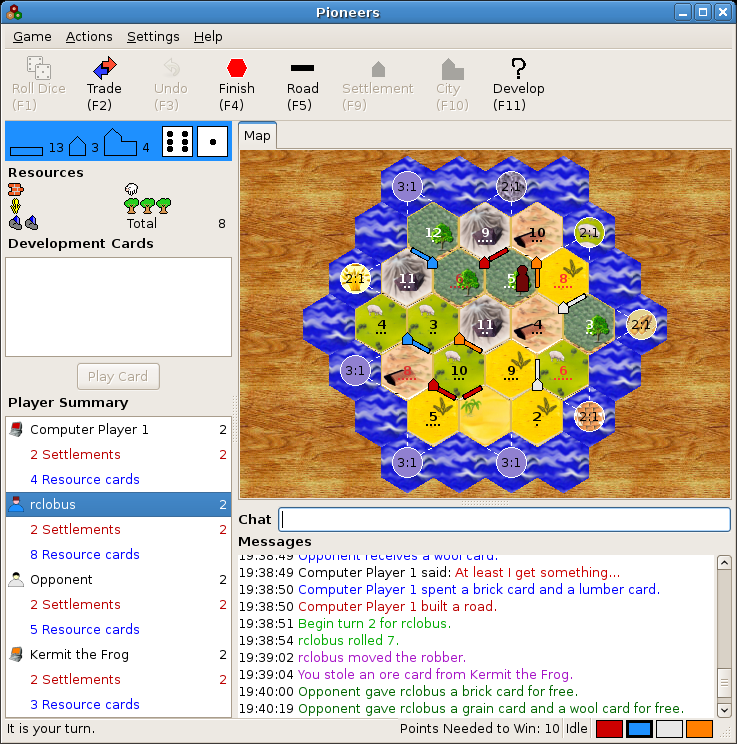
\includegraphics[width=\linewidth]{pioneers.png}
  \end{center}
  \caption{Zrzut ekranu z gry Pioneers}
  \label{pioneers}
\end{figure}

\subsection{JSettlers}
Aplikacja napisana w całości w Javie, rozwijana od początku 2004 roku,
dostępna na licencji GNU GPL\cite{jsettlers}. Aplikacja przystosowana
do uruchamiania w przeglądarce internetowej z zainstalowanym
środowiskiem uruchomieniowym Javy (\emph{ang. Java Runtime
  Environment}). Na \imref{jsettlers} został przedstawiony zrzut
ekranu z gry \emph{JSettlers}.

\begin{figure}[ht]
  \begin{center}
    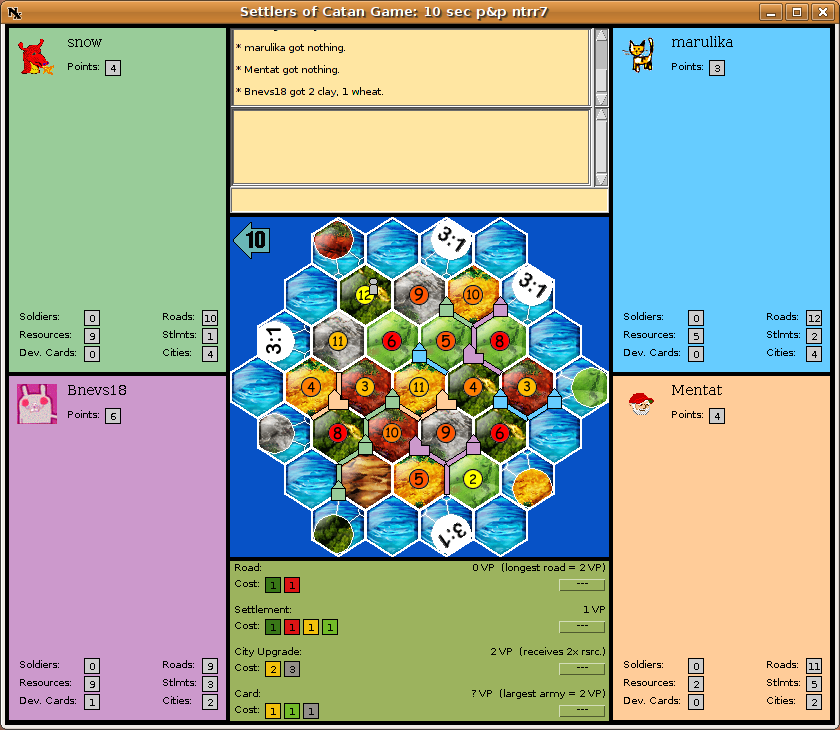
\includegraphics[width=\linewidth]{jsettlers.png}
  \end{center}
  \caption{Zrzut ekranu z gry JSettlers}
  \label{jsettlers}
\end{figure}

\subsection{Solito Server, MSN Games, PlayCatan.com}
Wszystkie te rozwiązania są oprogramowaniem własnościowym, w przypadku
dwóch ostatnich tytułów, płatnym. \emph{Solito Server} napisany został
przy użyciu technologii \emph{Adobe Flash}, dlatego jest w pewnym
stopniu uniezależniony od platformy sprzętowej (można go używać na
wszystkich platformach, na których dostępny jest \emph{Adobe
  Flash}). Pozostałe tytuły to oprogramowanie działające wyłącznie pod
kontrolą systemu operacyjnego \emph{Microsoft Windows}, wymagające
dodatkowo instalacji.

\subsection{Catan - The First Island}
Jest to prawdopodobnie jedyna implementacja gry dedykowana urządzeniom
mobilnym. Pierwotnie aplikacja napisana została w Javie dla urządzeń
mobilnych, przez niemiecką firmę \emph{Exozet Games}. W połowie 2009
roku pojawiła się także wersja przeznaczona dla konsoli \emph{Nintendo
  DS}. Oba rozwiązania umożliwiają rozgrywkę z graczem komputerowym
(\emph{AI}) oraz z innymi graczami poprzez \emph{Bluetooth} lub
\emph{WiFi}. Nie posiadają one niestety żadnego centralnego
serwera. Obie opisywane wersje są płatnym oprogramowaniem
własnościowym.

\clearpage

\section{Określenie funkcji aplikacji i wybór technologii}
Projektowana aplikacja składać się będzie z dwóch części: serwera i
klienta. Aplikacja w założeniu będzie wymagać bardzo dużego nakładu
pracy, w tym zaprojektowania interfejsu graficznego. Aby umożliwić
rozwój aplikacji, zdecydowałem się udostępnić całość kodu jako wolne
oprogramowanie na zasadach Powszechnej Licencji Publicznej GNU Affero
w wersji 3\cite{affero}.

Do zaimplementowania części serwerowej aplikacji zostanie wykorzystany
język \emph{Ruby} i framework \emph{Ruby on Rails}. Wybór można
uzasadnić bardzo dobrym wsparciem frameworka dla architektury
\emph{REST}, która zostanie wykorzystana do utworzenia \emph{API}.

\subsection{Ruby}
Język \emph{Ruby} został stworzony w 1995 roku przez Yukihiro
Matsumoto. Inspirowany jest on w głównej mierze językami, takimi jak:
\emph{Lisp}, \emph{Perl}, \emph{Python}, \emph{Smalltalk}, a także
\emph{CLU} i \emph{Eiffel}. Jest to wieloparadygmatowy, dynamicznie
typowany, interpretowany język programowania bardzo wysokiego poziomu
(ang. \emph{VHLL}\footnote{VHLL - very high-level programming
  language})\cite{ruby}. Najważniejszymi cechami języka są:

\begin{itemize}
\item pełna obiektowość - nie ma podziału na typy proste (wbudowane) i
  złożone. Pełnoprawnymi obiektami są także klasy, metody, wyrażenia
  lambda, itp.
\item pseudoklasyczny mechanizm dziedziczenia jednobazowego
\item moduły oferujące mechanizm zastępujący dziedziczenie wielobazowe
  (ang. \emph{mixin})
\item otwarte klasy, pozwalające na zmianę w dowolnym momencie
  wykonywania programu właściwości zdefiniowanych już klas (włącznie z
  klasami pochodzącymi z biblioteki standardowej języka)
\item \emph{monkey patching} - wykorzystanie mechanizmu otwartych klas
  do zmiany działania już istniejącego kodu w czasie wykonywania
  programu
\item metaprogramowanie - mechanizm ten umożliwia tworzenie kodu,
  który generuje kod w czasie wykonywania programu
\item ,,kacze typowanie'' - typy obiektów przekazywanych jako
  argumenty funkcji nie są w żaden sposób sprawdzane. Dzięki temu nie
  jest konieczne tworzenie skomplikowanych hierarchii dziedziczenia
  klas, wystarczy jedynie zaimplementować w klasach pewien wspólny
  podzbiór właściwości wymaganych przez wywoływaną na nich funkcję
\item domknięcia - mechanizm wiązania tworzonych funkcji z ich
  otoczeniem. Podczas wywołania funkcji ma ona dostęp do zmiennych,
  które zostały dowiązane do niej podczas jej tworzenia (nawet jeśli
  są one niedostępne podczas jej wywołania)
\item przejrzysta, czytelna składnia
\item bogata biblioteka standardowa
\end{itemize}

Język \emph{Ruby} doczekał się wielu różnych implementacji, z których
najbardziej dojrzałe są:

\begin{itemize}
\item \emph{Matz's Ruby Interpreter} (\emph{MRI}) - intepreter
  napisany w języku \emph{C}, uznawany \emph{de facto} za
  implementację referencyjną
\item \emph{JRuby} - interpreter napisany w języku Java, uruchamiany w
  \emph{wirtualnej maszynie Javy}
\end{itemize}

Głównym wskaźnikiem świadczącym o dojrzałości interpretera jest
możliwość uruchomienia na nim frameworka \emph{Ruby on
  Rails}. Wymienione wyżej implementacje najczęściej wykorzystywane są
do budowy środowisk produkcyjnych. Pozostałe implementacje są w
większości w fazie rozwoju, zaliczają się do nich
m.in. \emph{Cardinal}, \emph{IronRuby}, \emph{MacRuby}, \emph{MagLev},
\emph{Rubinius}, \emph{Ruby.NET} oraz \emph{XRuby}.

Ogromną zaletą języka \emph{Ruby} jest fakt, iż wszystkie wyżej
wymienione implementacje, za wyjątkiem \emph{MagLev}, to wolne
oprogramowanie. Rozwojem języka kieruje społeczność, tworząca kod
\emph{MRI}, nie jest on uzależniony od żadnych zewnętrznych firm (jak
ma to miejsce w przypadku języka \emph{Java} i firmy \emph{Sun
  Microsystems}).

W związku z tym, że język \emph{Ruby} utożsamiany jest głównie z
technologiami webowymi, należałoby nadmienić fakt, iż tworzenie
aplikacji internetowych nie miało wpływu na rozwój tego języka (tak
jak ma to miejsce w przypadku języka \emph{PHP}). Zamierzeniem
Yukihiro Matsumoto było stworzenie języka, który byłby
,,skuteczniejszy niż \emph{Perl} oraz bardziej zorientowany obiektowo
niż \emph{Python}''\cite{matzinterview}. Język \emph{Ruby} posiada
bardzo bogatą bibliotekę standardową, a także dużą ilość bibliotek
zewnętrznych (tzw. \emph{gemów}). Równie dobrze nadaje się do
tworzenia aplikacji okienkowych, serwerów sieciowych, jak i skryptów
systemowych. Nie zmienia to jednak faktu, że popularność języka wiąże
się nierozłącznie z frameworkiem \emph{Ruby on Rails}.

\subsection{Ruby on Rails}
Twórcą frameworka \emph{Ruby on Rails} jest duński programista David
Heinemeier Hansson. Framework powstał w wyniku prac nad aplikacją
\emph{Basecamp}, został udostępniony w połowie 2004 roku. Wzrost
popularności \emph{Ruby on Rails} nastąpił po ogłoszeniu przez firmę
\emph{Apple Inc.}, że będzie on dostarczany wraz z systemem \emph{Mac
  OS X v10.5 ''Leopard''}\cite{rubyonrails}. Swoje ogromne możliwości
framework zawdzięcza wykorzystaniu takich cech języka, jak
metaprogramowanie, kacze typowanie, czy możliwość otwierania klas.

Framework \emph{Ruby on Rails} umożliwia tworzenie aplikacji
internetowych w oparciu o wzorzec \emph{MVC}\footnote{MVC -
  model-widok-kontroler (ang. Model-View-Controller), wzorzec
  projektowy, którego założeniem jest podział aplikacji na modele,
  widoki i kontrolery. Podział jest realizowany w taki sposób, aby
  modyfikacja jednego elementu miała jak najmniejszy wpływ na
  działanie pozostałych}. \emph{Ruby on Rails} obsługuje wszystkie
popularne silniki bazodanowe poprzez bibliotekę mapowania
obiektowo-relacyjnego \emph{ActiveRecord}. Aplikacje napisane przy
użyciu frameworka mogą być uruchamiane na serwerach webowych, takich
jak \emph{Apache}, \emph{Lighttpd}, \emph{Abyss}, \emph{Thin},
\emph{Mongrel}. W przypadku zastosowania \emph{JRuby}, mogą być to
m.in. serwery aplikacji \emph{JBoss}, \emph{GlassFish} lub
\emph{Apache Geronimo}.

Cały framework jest udostępniony na zasadach licencji \emph{MIT}
\cite{mit}.

\subsubsection{Architektura Ruby on Rails}
Framework \emph{Ruby on Rails} składa się z komponentów, z których
główne to:

\begin{itemize}
\item \emph{ActiveRecord} - biblioteka mapowania
  obiektowo-relacyjnego, która powstała na podstawie wzorca
  projektowego o tej samej nazwie. Biblioteka ta oferuje znacznie
  więcej, niż wynika z implementowanego wzorca, m.in. różne rodzaje
  asocjacji (w tym asocjacje polimorficzne), mechanizm dziedziczenia
  jednotabelowego (\emph{STI}\footnote{STI - dziedziczenie
    jednotabelowe (ang. Single Table Inheritance) - technika
    umożliwiająca odzwierciedlenie w jednej tabeli relacyjnej bazy
    danych obiektów wielu dziedziczących po sobie klas})
  oraz walidatory
\item \emph{ActionPack} - biblioteka umożliwiająca tworzenie
  kontrolerów i widoków, odpowiada również za kierowanie zapytań do
  odpowiednich akcji kontrolerów (tzw. \emph{routing})
\item \emph{ActiveSupport} - biblioteka dodająca wiele użytecznych
  funkcji do klas biblioteki standardowej, ułatwiających tworzenie
  aplikacji webowych (i nie tylko)
\item \emph{ActionMailer} - biblioteka służąca do wysyłania wiadomości
  e-mail, np. poprzez zewnętrzne serwery \emph{SMTP}
\item \emph{ActiveResource} - biblioteka umożliwiająca mapowanie
  zasobów \emph{REST}\footnote{REST - ang. Representational State
    Transfer} na modele w aplikacji
\end{itemize}

Uproszczony diagram przedstawiający interakcje pomiędzy poszczególnymi
elementami frameworka został przedstawiony na
\imref{railsarchitecture}.

\begin{figure}[ht]
  \begin{center}
    \includegraphics[width=\linewidth]{railsarchitecture.png}
  \end{center}
  \caption{Architektura Ruby on Rails}
  \label{railsarchitecture}
\end{figure}

\subsubsection{Rozwój Ruby on Rails}
Na początku roku 2008 światło dzienne ujrzał nowy framework do
tworzenia aplikacji webowych o nazwie \emph{Merb}, silnie inspirowany
przez \emph{Ruby on Rails}. Został on stworzony z inicjatywy Ezry
Zygmuntowicza, założyciela firmy \emph{Engine Yard}. W założeniach
oprogramowanie miało być szybsze i bardziej modularne niż jego
pierwowzór. Spory pomiędzy zwolennikami nowopowstałego frameworka a
dotychczasową społecznością spowodowały powstanie w niej pewnego
rodzaju rozłamu. Przy narastającej fali krytyki z obu stron, niedługo
po wydaniu \emph{Merba 1.0}, David Heinemeier Hansson ogłosił
połączenie obu grup programistów\cite{merge}. Utworzony zespół miał
się zająć połączeniem powstającego \emph{Merba 2} i \emph{Ruby on
  Rails 3}. Zgodnie z ustaleniami, pierwsze wydania \emph{Ruby on
  Rails 3} mają się pojawić pod koniec 2009 roku.

\subsection{JavaScript}
Język \emph{JavaScript} powstał pod koniec 1995 roku w firmie
\emph{Netscape Communications Corporation} jako alternatywa dla
uruchamianych w przeglądarce apletów \emph{Javy}. Jego twórcą jest
amerykański programista Brendan Eich. Począwszy od 1996 roku, język
jest standaryzowany przez \emph{ECMA International}\footnote{ECMA -
  Europejskie Stowarzyszenie na rzecz Standaryzacji Systemów
  Informacyjnych i Komunikacyjnych (ang. European association for
  standardizing information and communication systems), organizacja
  zajmująca się standaryzacją systemów informatycznych w Europie} jako
\emph{ECMAScript}.
\label{javascript}

Pomimo swojej nazwy jasno kojarzącej się z językiem \emph{Java}, język
\emph{JavaScript} jest (z wyjątkiem kilku elementów) językiem
diametralnie od \emph{Javy} różnym. Największy wpływ na jego rozwój
miały języki takie jak: \emph{Self}, \emph{C}, \emph{Scheme},
\emph{Perl} oraz \emph{Python}. Aby upodobnić język do błyskawicznie
zyskującej wówczas popularność \emph{Javy}, zapożyczony został zestaw
słów kluczowych i składnia. Ta prosta marketingowa sztuczka
zaowocowała całkowitym niezrozumieniem tego języka przez programistów,
którzy przez wiele lat traktowali go jako pewien podzbiór języka
\emph{Java}. W rzeczywistości, język \emph{JavaScript} jest znacznie
bliżej spokrewniony z językami funkcyjnymi, takimi jak \emph{Lisp}.

Interpreter \emph{JavaScriptu} wbudowany jest w niemal każdą
współczesną przeglądarkę internetową, co czyni go jednym z najbardziej
rozpowszechnionych języków programowania na świecie.

Najważniejszymi cechami języka, odróżniającymi go od języków
,,c-pochodnych'' (w tym od \emph{Javy}) są:

\begin{itemize}
\item dynamiczne typowanie
\item domknięcia
\item prawie całkowita obiektowość - występuje podział na typy proste
  i obiekty. Obiekty są tablicami asocjacyjnymi, ich właściwości można
  dowolnie modyfikować podczas wykonania programu (w praktyce
  mechanizm ten jest bardzo podobny do ,,otwierania klas'' w języku
  \emph{Ruby}).
\item dziedziczenie prototypowe - mechanizm dziedziczenia
  bezklasowego. Jedyną cechą umożliwiającą stwierdzenie pokrewieństwa
  obiektów jest posiadanie przez nie wspólnego prototypu
\end{itemize}

Główne implementacje \emph{JavaScriptu} to:

\begin{itemize}
\item \emph{SpiderMonkey} - pierwszy interpreter, napisany przez
  twórcę języka w \emph{C}, wykorzystywany m.in. w przeglądarce \emph{Mozilla
    Firefox}.
\item \emph{Rhino} - interpreter napisany w \emph{Javie}, pozwala na
  uruchamianie \emph{JavaScriptu} na wirtualnej maszynie \emph{Javy}
\item \emph{KDE's JavaScript engine} - wykorzystywany w przeglądarce
  \emph{Konqueror}
\item \emph{WebKit} - napisany w \emph{C++} interpreter używany
  m.in. w przeglądarce \emph{Safari} firmy \emph{Apple Inc.}
\item \emph{V8} - zaimplementowany w \emph{C++} interpreter używany w
  przeglądarce \emph{Google Chrome}
\end{itemize}

Rozmaite dialekty \emph{JavaScriptu} (a dokładniej standardu
\emph{ECMAScript}) znalazły się także poza przeglądarkami
internetowymi. Wśród nich wyróżnić można m.in.:

\begin{itemize}
\item \emph{JScript} - dialekt stworzony i rozwijany przez firmę
  \emph{Microsoft}. Oprócz wbudowania w przeglądarkę \emph{Microsoft
    Internet Explorer} interpreter tego dialektu jest również częścią
  środowiska \emph{Microsoft Windows Scripting Host}, jest to także
  jeden z podstawowych języków środowiska \emph{.NET}
\item \emph{ActionScript} - dialekt rozwijany przez firmę \emph{Adobe
    Systems}, wykorzystywany w środowisku \emph{Adobe Flash}
\end{itemize}

\subsubsection{XMLHttpRequest (Ajax)}
Po rozpowszechnieniu się \emph{JavaScriptu} w przeglądarkach
internetowych, był on używany głównie do ,,upiększania'' stron
\emph{HTML} i dodawania do nich dynamicznych elementów. Stał się swego
rodzaju dodatkiem, ułatwiającym korzystanie ze stron.

Sytuacja zaczęła się zmieniać po wprowadzeniu przez firmę
\emph{Microsoft} obiektu \emph{ActiveX} nazwanego \emph{XMLHTTP} w
przeglądarce \emph{Microsoft Internet Explorer 5}. Najważniejszą cechą
tego mechanizmu była możliwość komunikacji z serwerem bez konieczności
przeładowywania całego dokumentu. W krótkim czasie podobne rozwiązania
zostały zaimplementowane w konkurencyjnych przeglądarkach, m.in.w
\emph{Mozilli} i \emph{Safari}. Pomimo tego, że funkcje te były
dostępne w przeglądarkach od końca 1999 roku, pierwsze duże aplikacje
zaczęły z nich korzystać dopiero w 2004 roku. Najważniejszymi
aplikacjami, które spopularyzowały opisywany mechanizm były
\emph{Gmail} i \emph{Google Maps}, należące do firmy \emph{Google
  Inc.} W 2005 roku wprowadzony został termin \emph{Ajax}
(ang. asynchronous JavaScript and XML), oznaczający wykorzystanie
języków \emph{JavaScript} i \emph{XML} do asynchronicznej komunikacji
z serwerem\footnote{w rzeczywistości jednak, żaden z wymienionych
  elementów nie jest wymagany. W niektórych przeglądarkach zamiast
  \emph{JavaScriptu} można użyć innego języka (np. \emph{VBScript}),
  zamiast \emph{XML}-a często jest używany \emph{JSON} lub zwykły
  tekst, a zapytania wcale nie muszą być asynchroniczne}.

W związku z ograniczeniami narzucanymi przez przeglądarki internetowe,
wszystkie zapytania wykonywane przy pomocy skryptów muszą odwoływać
się do domeny, z której pobrany został dokument
\emph{HTML}\cite{origin} (ang. same origin policy). Dla aplikacji
wymagających komunikacji z różnymi domenami (np. ściągającymi dane z
innych aplikacji) powstało rozwiązanie nazwane \emph{JSONP}. W
uproszczeniu polega ono na dodawaniu do kodu dokumentu \emph{HTML}
tagu \texttt{<script>}. Tag ten może zostać dodany z wnętrza
działającego w przeglądarce skryptu, spowoduje on załadowanie i
zinterpretowanie przez przeglądarkę kodu pochodzącego z dowolnej
domeny. Rozwiązanie to jest używane do przesyłania danych w formacie
\emph{JSON}. Przesyłany obiekt musi być otoczony wywołaniem funkcji
zwrotnej (ang. callback), w celu poinformowania skryptu o otrzymaniu
danych. Podobne rozwiązanie jest używane również do tzw. leniwego
ładowania kodu aplikacji (dynamiczne ładowanie zależności). Należy
zaznaczyć, że ładowanie kodu z innych domen jest potencjalnie
niebezpiecznym działaniem i powinno być wykorzystywane z dużą rozwagą.

\subsubsection{HTTP Push (Comet)}
W przypadku standardowego wykorzystania technologii \emph{Ajax},
przesyłanie danych odbywa się na żądanie przeglądarki internetowej. W
niektórych rozwiązaniach taki mechanizm jest zbyt mało wydajny i
wprowadza w komunikacji niepożądane opóźnienia. Najprostszym
przykładem takiej aplikacji jest czat. W klasycznym rozwiązaniu każdy
klient musi co pewien czas odpytywać serwer o to, czy pojawiły się na
nim jakieś nowe wiadomości. Im mniejszy jest czas pomiędzy
poszczególnymi zapytaniami, tym większa jest ilość wykonywanych
zapytań i co za tym idzie, tym większe jest obciążenie
serwera. Technika ta jest także nazywana \emph{HTTP
  Pull}\footnote{ang. pull technology, client pull - styl komunikacji
  sieciowej, w którym wszystkie połączenia są inicjowane przez
  klienta\cite{pull}}, schemat jej działania został przedstawiony na
\imref{pull}.

\begin{figure}[ht]
  \begin{center}
    \includegraphics[width=\linewidth]{pull.pdf}
  \end{center}
  \caption{Schemat działania mechanizmu odpytywania (\emph{HTTP
      Pull})}
  \label{pull}
\end{figure}

Jeśli przyjrzeć się bliżej aplikacji takiej jak \emph{Gmail}, okazuje
się, że nie wykonuje ona cyklicznego odpytywania serwera, a wszystkie
dane przesyłane są do klienta niemalże bez opóźnień. Najprostszym
sposobem na uniknięcie częstego odpytywania serwera jest zastosowanie
mechanizmu wydłużonego odpytywania (ang. long polling). Polega on na
wydłużaniu czasu trwania zapytań poprzez opóźnianie reakcji
serwera. Jeśli po otrzymaniu zapytania na serwerze nie ma żadnych
danych do pobrania, zamiast wysyłać informację o braku danych serwer
wstrzymuje się z odpowiedzią do czasu ich nadejścia. W przypadku, gdy
na serwerze pojawią się dane, są one natychmiast wysyłane do klienta
poprzez otwarte połączenie. W przypadku, gdy zostanie przekroczony
maksymalny czas trwania połączenia (ang. timeout) jest ono zamykane. W
obu przypadkach klient natychmiastowo wywołuje kolejne zapytanie,
które ponownie oczekuje na pojawienie się danych. Schemat działania
takiego mechanizmu został przedstawiony na \imref{longpolling}.

\begin{figure}[ht]
  \begin{center}
    \includegraphics[width=\linewidth]{longpolling.pdf}
  \end{center}
  \caption{Schemat działania mechanizmu wydłużonego odpytywania}
  \label{longpolling}
\end{figure}

Niewątpliwą wadą przedstawionego rozwiązania jest fakt, iż w
przypadku, gdy dane pojawiają się na serwerze z dużą częstotliwością,
wywoływanych jest dużo pojedynczych zapytań. Skutkuje to oczywiście
wzrostem obciążenia serwera. W mechanizmie wydłużonego odpytywania
wykorzystywane są asynchroniczne zapytania \emph{XMLHttpRequest}. W
przypadku pobierania danych z innych domen wykorzystywany jest
mechanizm \emph{JSONP}.

Innym, bardziej wyrafinowanym sposobem komunikacji poprzez \emph{HTTP
  Push} jest strumieniowanie danych. Do strumieniowania danych
wykorzystywany jest fakt, iż wszystkie współczesne przeglądarki
internetowe renderują strony progresywnie. W związku z tym, możliwe
staje się wywołanie ,,nieskończonego'' zapytania, które będzie
interpretowane przez silnik na bieżąco, w chwili pojawiania się nowych
elementów. Do wykonania takiego zapytania wykorzystywany jest ukryty
znacznik \texttt{<iframe>}. Znacznik ten umożliwia zagnieżdżenie w
dokumencie innego dokumentu, pochodzącego z innego adresu
internetowego\footnote{w tym przypadku również nie jest możliwe
  załadowanie dokumentu z innej domeny, zgodnie z polityką
  bezpieczeństwa przeglądarek}. Podobnie jak w przypadku \emph{JSONP}
przesyłane dane muszą być otoczone wywołaniem funkcji, która ma je
odebrać. Dodatkowo całość musi zostać otoczona znacznikiem
\texttt{<script>}. Każdy taki znacznik jest renderowany
(interpretowany) przez przeglądarkę zaraz po jego otrzymaniu. W
przypadku, gdy na serwerze nie ma żadnych danych, wysyłany jest co
pewien czas pusty znacznik, w celu utrzymania połączenia. Schemat
działania mechanizmu strumieniowania został przedstawiony na
\imref{streaming}.

\begin{figure}[ht]
  \begin{center}
    \includegraphics[width=\linewidth]{streaming.pdf}
  \end{center}
  \caption{Schemat mechanizmu strumieniowania danych}
  \label{streaming}
\end{figure}

W związku z tym, że opisywane mechanizmy wykorzystują techniki
nieobjęte żadną specyfikacją, ich działanie jest w dużej mierze
zależne od implementacji poszczególnych przeglądarek
internetowych. Największym wyzwaniem jest przystosowanie wymienionych
technik do przeglądarek w urządzeniach mobilnych. Okazuje się również,
że użycie \emph{HTTP Push} na powszechnie używanych serwerach
\emph{HTTP} jest wysoce nieefektywne lub wręcz niemożliwe. Niemal
wszystkie dostępne rozwiązania wymagają uruchomienia dodatkowych
serwerów, odpowiedzialnych wyłącznie za obsługę \emph{HTTP Push}. Są
to serwery takie jak: \emph{Caplin Liberator}, \emph{Cometd},
\emph{ErlyComet}, \emph{GlassFish}, \emph{Jetty},
\emph{Lightstreamer}, \emph{Meteor}, \emph{Orbited}, \emph{Persevere}
i \emph{RMDS2Web Server}\cite{cometmaturity}. Dodatkową przeszkodą w
komunikacji przeglądarki z dodatkowym serwerem jest opisywane już
wcześniej zabezpieczenie \emph{same origin policy}. Całość komplikuje
również fakt, że przeglądarki internetowe realizują te zabezpieczenia
w różny sposób\cite{xssinfo}.

Wszystkie opisywane w tym rozdziale techniki noszą wspólną nazwę
\emph{Comet}\cite{comet}. W 2007 roku organizacja \emph{DOJO
  Foundation}\footnote{DOJO Foundation - niedochodowa
  (ang. non-profit) organizacja zajmująca się promocją biblioteki
  \emph{Dojo Toolkit}} podjęła się również próby ustandaryzowania tych
rozwiązań pod nazwą \emph{protokołu Bayeux}\cite{bayeux}. Alternatywą
dla \emph{Cometa} jest stosowanie rozwiązań pochodzących z apletów
\emph{Javy} lub aplikacji \emph{Adobe Flash}, które mogą samodzielnie
nawiązywać połączenia \emph{TCP} (bez udziału przeglądarki
internetowej). Powstająca specyfikacja języka \emph{HTML 5} zawiera
również rozwiązanie nazwane \emph{Web Sockets API}, które umożliwia
dwustronną komunikację z serwerem \emph{HTTP}\cite{websockets}.

\subsubsection{DOM}
Obiektowy model dokumentu(ang. Document Object Model) jest konwencją
reprezentacji dokumentów \emph{XML}, \emph{XHTML} i \emph{XML} w
postaci modelu obiektowego. Jest on wymagany przez język
\emph{JavaScript} do odczytywania i modyfikowania struktury dokumentu
z poziomu kodu. Jest to zdecydowanie najbardziej niespójny element
współczesnych przeglądarek. Ma to związek m.in. z tym, że pierwsze
próby ustandaryzowania tego rozwiązania odbyły się w 1997 roku, a
standard wszedł w powszechne użycie dopiero około roku
2000. Niespójności te są na tyle duże, że pisząc nawet prosty skrypt
odwołujący się bezpośrednio do \emph{DOM-u} przeglądarki, możemy
spodziewać się, że nie będzie on przenośny. Dostosowywanie kodu do
różnic występujących w poszczególnych przeglądarkach jest wyjątkowo
żmudnym i czasochłonnym zadaniem. W praktyce okazuje się, że pisanie
kodu operującego bezpośrednio na dokumencie jest zjawiskiem stosunkowo
rzadkim. W większości przypadków wykorzystuje się do tego celu gotowe
biblioteki, zapewniające pewien poziom abstrakcji w dostępie do
\emph{DOM-u}, przenośność kodu pomiędzy różnymi przeglądarkami oraz
poprawiające użyteczność samego
\emph{JavaScriptu}. Najpopularniejszymi bibliotekami tego typu są:
\emph{jQuery}, \emph{Prototype}, \emph{DOJO Toolkit}, \emph{Yahoo!
  User Interface Library} oraz \emph{Google Web Toolkit}.

\subsection{REST}
\emph{REST} to styl architektury oprogramowania systemów
rozproszonych. Skrót ten pochodzi od ang. \emph{Representational State
  Transfer}, został wprowadzony w pracy doktorskiej Roya Fieldinga
pt. ,,Architectural Styles and the Design of Network-based Software
Architectures''\cite{rest}. Jednym z założeń \emph{REST}, jest
komunikacja serwera z klientem przy pomocy bezstanowych
połączeń. Wszystkie informacje przechowywane na serwerze udostępniane
są w postaci zasobów, posiadających ściśle określone
identyfikatory. Na każdym z zasobów możliwe jest wykonanie
podstawowych operacji: utworzenia, odczytania, aktualizacji i
usunięcia (tzw. \emph{CRUD}\footnote{ang. create, read, update and
  delete}). W przypadku protokołu \emph{HTTP} akcje te, mapowane są na
odpowiadające im metody \emph{HTTP}, zwykle są to: \emph{POST},
\emph{GET}, \emph{PUT} i \emph{DELETE}\cite{agile}.

Główną cechą mającą silny wpływ na rosnącą popularność \emph{REST}
jest prostota użytkowania, przez co stopniowo wypierane są rozwiązania
oparte o \emph{XML-RPC} czy \emph{SOAP}. Dobrym przykładem ukazania
tego faktu jest \emph{Amazon Web Services}. Klienci tych usług mają
swobodny wybór pomiędzy dostępem do nich poprzez interfejs \emph{REST}
i \emph{SOAP}, jednak 80\% z nich decyduje się na użycie
\emph{REST}\cite{awsblog}.

Począwszy od wersji 1.2, framework \emph{Ruby on Rails} w pełni
wspiera \emph{REST}. Od wersji 2.0 jest to domyślny i zalecany sposób
tworzenia aplikacji w tym frameworku.

\clearpage

\section{Projektowanie aplikacji}

\subsection{Plansza}\label{sec:board}
Jednym z podstawowych problemów, jakie należy rozwiązać projektując
aplikację, jest przechowywanie planszy w relacyjnej bazie
danych. Naturalnie, pierwszym pomysłem było wykorzystanie mechanizmu z
działającego rozwiązania, a mianowicie z gry \emph{Pioneers}.

Plansza do gry w ,,Osadników'' składa się w pierwotnej wersji z 37
połączonych ze sobą sześciokątów. Niektóre ich wierzchołki i krawędzie
przeznaczone są pod budowę dróg i osad. Sytuację najbardziej
komplikuje fakt, iż większość wierzchołków i krawędzi jest wspólna dla
kilku połączonych sześciokątów. Rozwiązanie zastosowane w grze
\emph{Pioneers} polega na ułożeniu wszystkich sześciokątów na planszy
w dwuwymiarowej tablicy. Dodatkowo każdy z nich posiada dwie
sześcioelementowe tablice wskaźników, wskazujących na odpowiednie
wierzchołki i krawędzie. Przy tworzeniu wierzchołka lub krawędzi
ustawiane są odpowiednie wskaźniki w sąsiadujących sześciokątach. To
stosunkowo proste rozwiązanie okazuje się być trudne w realizacji w
relacyjnej bazie danych. Przykładowe połączenie sześciokąta z
wierzchołkami wymagałoby użycia sześciu kluczy obcych lub utworzenia
dodatkowej tabeli łączącej. Rozwiązanie takie wprowadza do bazy dużo
niepotrzebnych połączeń i jest mało wydajne.

Jednym z działań, które gracz może wykonać podczas gry, jest
zbudowanie przez niego osady. Do sprawdzenia poprawności współrzędnych
budowanej osady niezbędnych jest wykonanie kilku czynności:

\begin{itemize}
\item sprawdzenie, czy na jednym z sąsiadujących wierzchołków nie
  znajduje się już inna osada - minimalna odległość pomiędzy osadami
  wynosi dwie drogi (dwie krawędzie)
\item sprawdzenie, czy na jednej z sąsiadujących krawędzi wybudowana
  jest droga należąca do gracza - budowane osady muszą być połączone
  drogami
\item sprawdzenie, czy jeden z sąsiadujących sześciokątów jest
  lądem. Osady nie mogą być budowane na brzegach planszy (na
  ,,morzu'')
\end{itemize}

Bardzo podobne czynności musimy wykonać, aby stwierdzić poprawność
współrzędnych budowanej przez gracza drogi. Okazuje się więc, że
najczęściej wykonywaną operacją jest pobranie sąsiadujących
(dołączonych) elementów planszy. Najlepiej więc, gdyby na podstawie
współrzędnych budowanej osady można było łatwo wyliczyć zbiór
współrzędnych dołączonych do wierzchołka sześciokątów, wierzchołków i
krawędzi. Aby ułatwić przekształcenia, wszystkie elementy planszy
muszą być jednoznacznie identyfikowalne na podstawie dwóch
współrzędnych.

Oprócz zbioru sześciokątów, wierzchołków i krawędzi, plansza do gry
powinna zawierać informacje o jej rozmiarze (ilości wierszy i kolumn)
oraz o aktualnym położeniu ,,rozbójnika''.

\subsubsection{Sześciokąty}
Podobnie jak w implementacji gry \emph{Pioneers}, sześciokąty zostały
ułożone w dwuwymiarową tablicę. Każdy z nich ma przypisaną pozycję,
składającą się z numeru wiersza $x$ i kolumny $y$. Sposób numeracji
sześciokątów został przedstawiony na \imref{board}. Dodatkowo, każdy
sześciokąt powinien zawierać następujące informacje:

\begin{itemize}
\item typ - sześciokąt może reprezentować wzgórze, pole uprawne, las,
  pastwisko, górę, pustynię lub morze
\item wynik rzutu kością, po wyrzuceniu którego pole przynosi
  dochód; sześciokąty reprezentujące morze i pustynię nie posiadają
  żadnej wartości
\item pozycję (kierunek) i rodzaj szlaku handlowego - cecha ta dotyczy
  wyłącznie niektórych sześciokątów reprezentujących morze
\end{itemize}

\begin{figure}[ht]
  \begin{center}
    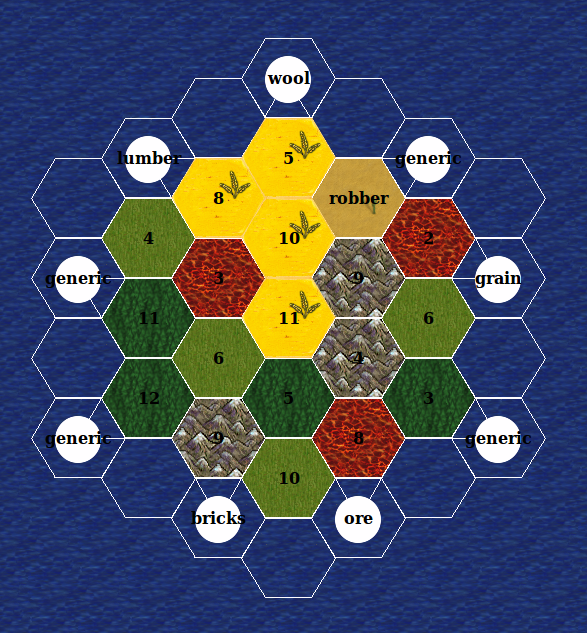
\includegraphics[width=\linewidth]{board.pdf}
  \end{center}
  \caption{Zasada numerowania sześciokątów na planszy}
  \label{board}
\end{figure}

\subsubsection{Wierzchołki}
Numerowanie wierzchołków jest nieco bardziej skomplikowanym
zadaniem. Wykorzystany został tutaj fakt, iż, przy numeracji
sześciokątów przedstawionej na \imref{board}, w każdym z nich można
wyróżnić wierzchołki ,,górne'' (posiadające numer wiersza taki jak
numer wiersza sześciokąta) i ,,dolne'' (posiadające numer wiersza o
jeden większy niż numer wiersza sześciokąta). Dla ujednolicenia
schematu numeracji, konieczne stało się ponumerowanie dodatkowych
pozycji, w których nie występują wierzchołki. Omawiany sposób
numeracji został przedstawiony na \imref{nodes}. Dla planszy o
rozmiarach $x$ wierszy i $y$ kolumn, otrzymujemy tablicę wierzchołków
posiadającą wysokość $x+1$ wierszy i szerokość $2y+2$ kolumn. Każdy
zasiedlony wierzchołek musi należeć do któregoś z graczy oraz posiadać
dodatkową informację o tym, czy jest osadą, czy miastem.

\begin{figure}[ht]
  \begin{center}
    \includegraphics[width=\linewidth]{nodes.pdf}
  \end{center}
  \caption{Zasada numerowania wierzchołków na planszy}
  \label{nodes}
\end{figure}

\subsubsection{Krawędzie}
Krawędzie numerowane są na podobnej zasadzie co wierzchołki. Również
niezbędne okazało się wprowadzenie niepowiązanych z sześciokątami
pozycji. Sposób numeracji krawędzi został przedstawiony na
\imref{edges}. Plansza o rozmiarach $x$ wierszy i $y$ kolumn, posiada
tablicę krawędzi o wysokości $x+1$ wierszy i szerokości $3y+4$
kolumn. Podobnie jak w przypadku wierzchołka -- zasiedlona krawędź
musi należeć do jednego z graczy.

\begin{figure}[ht]
  \begin{center}
    \includegraphics[width=\linewidth]{edges.pdf}
  \end{center}
  \caption{Zasada numerowania krawędzi na planszy}
  \label{edges}
\end{figure}

\subsubsection{Obliczanie pozycji elementów dołączonych}
\label{sec:calculations}
Po wprowadzeniu przedstawionych schematów numeracji, możliwe staje się
wyznaczenie pozycji elementów sąsiadujących z ponumerowanymi
sześciokątami, wierzchołkami i krawędziami. Zbiory dołączonych
sześciokątów $\text{hexes}_{adj}$, wierzchołków $\text{nodes}_{adj}$ i
krawędzi $\text{edges}_{adj}$ do danego sześciokąta o współrzędnych
$(x, y)$ zostały przedstawione kolejno w równaniach \ref{hexhexes},
\ref{hexnodes} i \ref{hexedges}. Każdy sześciokąt posiada po sześć
sąsiadujących pozycji elementów każdego typu.

\begin{equation}
  \begin{aligned}
    \text{hexes}_{adj}(\text{hex}_{x,y})=
    \{
    (x-1, y+1),
    (x-1, y),
    (x, y-1),\\
    (x+1, y-1),
    (x+1, y),
    (x, y+1)
    \}
  \end{aligned}
  \label{hexhexes}
\end{equation}
\begin{equation}
  \begin{aligned}
    \text{nodes}_{adj}(hex_{x,y})=\{
    (x+1, 2y),
    (x+1, 2y+1),
    (x+1, 2y+2),\\
    (x, 2y+3),
    (x, 2y+2),
    (x, 2y+1)
    \}
  \end{aligned}
  \label{hexnodes}
\end{equation}
\begin{equation}
  \begin{aligned}
    \text{edges}_{adj}(hex_{x,y})=\{
    (x+1, 3y+2),
    (x+1, 3y+4),
    (x, 3y+6),\\
    (x, 3y+5),
    (x, 3y+4),
    (x, 3y+3)
    \}
  \end{aligned}
  \label{hexedges}
\end{equation} \\

W przypadku wyznaczania elementów sąsiadujących z wierzchołkiem
sytuacja jest nieco bardziej skomplikowana. Zbiory elementów
dołączonych do danego wierzchołka są różne dla wierzchołków
znajdujących się w kolumnach parzystych i nieparzystych. Każdy ze
zbiorów składa się z trzech elementów. Zbiór sąsiadujących:
sześciokątów $\text{hexes}_{adj}$, wierzchołków $\text{nodes}_{adj}$ i
krawędzi $\text{edges}_{adj}$, z danym wierzchołkiem o współrzędnych
$(x, y)$, zostały przedstawione w równaniach \ref{nodehexes},
\ref{nodenodes} i \ref{nodeedges}.

\begin{equation}
  \text{hexes}_{adj}(\text{node}_{x,y})=
  \left\{
    \begin{array}{l r l}
      \begin{aligned}
      \{
      (x-1, \left\lfloor\frac{y}{2}\right\rfloor-1), \\
      (x-1, \left\lfloor\frac{y}{2}\right\rfloor), \\
      (x, \left\lfloor\frac{y}{2}\right\rfloor-1)
      \}
      \end{aligned} & \mbox{dla } y=2n, & n\in\mathbb{Z} \\[40pt]
      \begin{aligned}
        \{
        (x-1, \left\lfloor\frac{y}{2}\right\rfloor), \\
        (x, \left\lfloor\frac{y}{2}\right\rfloor-1), \\
        (x, \left\lfloor\frac{y}{2}\right\rfloor)
        \}
      \end{aligned} & y=2n+1, & n\in\mathbb{Z} \\
    \end{array} \right.
  \label{nodehexes}
\end{equation}
\begin{equation}
  \text{nodes}_{adj}(\text{node}_{x,y})=
  \left\{
    \begin{array}{l r l}
      \begin{aligned}
        \{
        (x-1, 3\left\lfloor\frac{y}{2}\right\rfloor+3), \\
        (x, 3\left\lfloor\frac{y}{2}\right\rfloor+3), \\
        (x, 3\left\lfloor\frac{y}{2}\right\rfloor+2)
        \}
      \end{aligned} & \mbox{dla } y=2n, & n\in\mathbb{Z} \\[40pt]
      \begin{aligned}
        \{
        (x, y+1), \\
        (x, y-1), \\
        (x+1, y-1)
        \}
      \end{aligned} & y=2n+1, & n\in\mathbb{Z} \\
    \end{array} \right.
  \label{nodenodes}
\end{equation}
\begin{equation}
  \text{edges}_{adj}(\text{node}_{x,y})=
  \left\{
    \begin{array}{l r l}
      \begin{aligned}
      \{
      (x-1, 3\left\lfloor\frac{y}{2}\right\rfloor+3), \\
      (x, 3\left\lfloor\frac{y}{2}\right\rfloor+3), \\
      (x, 3\left\lfloor\frac{y}{2}\right\rfloor+2)
      \}
      \end{aligned} & \mbox{dla } y=2n, & n\in\mathbb{Z} \\[40pt]
      \begin{aligned}
      \{
      (x, 3\left\lfloor\frac{y}{2}\right\rfloor+4), \\
      (x, 3\left\lfloor\frac{y}{2}\right\rfloor+2), \\
      (x, 3\left\lfloor\frac{y}{2}\right\rfloor+3)
      \}
      \end{aligned} & y=2n+1, & n\in\mathbb{Z} \\
    \end{array} \right.
  \label{nodeedges}
\end{equation} \\

Podobna sytuacja ma miejsce w przypadku wyliczania współrzędnych
elementów dołączonych do krawędzi. W tym przypadku dla trzech
następujących po sobie kolumn otrzymujemy trzy różne zbiory. Zbiory te
w przypadku dołączonych sześciokątów i wierzchołków składają się z
dwóch elementów, natomiast w przypadku krawędzi -- z czterech. Zbiory
sześciokątów $\text{hexes}_{adj}$, wierzchołków $\text{nodes}_{adj}$ i
krawędzi $\text{edges}_{adj}$, dla krawędzi o współrzędnych $(x,y)$,
zostały przedstawione w równaniach \ref{edgehexes}, \ref{edgenodes} i
\ref{edgeedges}.

\begin{equation}
  \text{hexes}_{adj}(\text{edge}_{x,y})=
  \left\{
    \begin{array}{l r l}
      \begin{aligned}
        \{
        (x, \left\lfloor\frac{y}{3}\right\rfloor-2), \\
        (x, \left\lfloor\frac{y}{3}\right\rfloor-1)
        \}
      \end{aligned} & \mbox{dla } y=3n, & n\in\mathbb{Z} \\[30pt]
      \begin{aligned}
        \{
        (x-1, \left\lfloor\frac{y}{3}\right\rfloor-1), \\
        (x, \left\lfloor\frac{y}{3}\right\rfloor-1)
        \}
      \end{aligned} & y=3n+1, & n\in\mathbb{Z} \\[30pt]
      \begin{aligned}
      \{
      (x-1, \left\lfloor\frac{y}{3}\right\rfloor), \\
      (x, \left\lfloor\frac{y}{3}\right\rfloor-1)
      \}
      \end{aligned} & y=3n+2, & n\in\mathbb{Z} \\
    \end{array} \right.
  \label{edgehexes}
\end{equation}
\begin{equation}
  \text{nodes}_{adj}(\text{edge}_{x,y})=
  \left\{
    \begin{array}{l r l}
      \begin{aligned}
      \{
      (x+1, 2\left\lfloor\frac{y}{3}\right\rfloor-2), \\
      (x, 2\left\lfloor\frac{y}{3}\right\rfloor-1)
      \}
      \end{aligned} & \mbox{dla } y=3n, & n\in\mathbb{Z} \\[30pt]
      \begin{aligned}
        \{
        (x, 2\left\lfloor\frac{y}{3}\right\rfloor-1), \\
        (x, 2\left\lfloor\frac{y}{3}\right\rfloor)
        \}
      \end{aligned} & y=3n+1, & n\in\mathbb{Z} \\[30pt]
      \begin{aligned}
      \{
      (x, 2\left\lfloor\frac{y}{3}\right\rfloor+1), \\
      (x, 2\left\lfloor\frac{y}{3}\right\rfloor)
      \}
      \end{aligned} & y=3n+2, & n\in\mathbb{Z} \\
    \end{array} \right.
  \label{edgenodes}
\end{equation}
\begin{equation}
  \text{edges}_{adj}(\text{edge}_{x,y})=
  \left\{
    \begin{array}{l r@{,~} l}
      \begin{aligned}
        \{
        (x+1, y-2), \\
        (x+1, y-1), \\
        (x, y+1), \\
        (x, y-1)
        \}
      \end{aligned} & \mbox{dla } y=3n & n\in\mathbb{Z} \\[40pt]
      \begin{aligned}
        \{
        (x-1, y+2), \\
        (x, y-2), \\
        (x, y-1), \\
        (x, y+1)
        \}
      \end{aligned} & y=3n+1 & n\in\mathbb{Z} \\[40pt]
      \begin{aligned}
        \{
        (x-1, y+1), \\
        (x, y-1), \\
        (x, y+2), \\
        (x, y+1)
        \}
      \end{aligned} & y=3n+2 & n\in\mathbb{Z} \\
    \end{array} \right.
  \label{edgeedges}
\end{equation}

\subsection{Gra}
Głównym zadaniem obiektów tej klasy będzie przechowywanie informacji o
stanie gry. Każda gra musi posiadać trzech lub czterech graczy oraz
planszę, na której toczy się rozgrywka. Ze względu na to, że przebieg
gry podzielony jest na etapy, a każdy z etapów składa się z wielu faz,
konieczne będzie zaimplementowanie maszyny stanowej. Dzięki maszynie
stanowej ,,fazy gry'', możliwe będzie sprawdzanie poprawności ruchów
wykonywanych przez graczy, oraz sterowanie przebiegiem gry.

\subsubsection{Maszyna stanowa ,,fazy gry''}
Gra ,,Osadnicy z Catanu'' podzielona jest na dwa etapy. Pierwszym
etapem gry jest etap zasiedlenia wyspy, podczas którego gracze kolejno
stawiają na planszy po jednej osadzie i drodze. Następnie każdy z
graczy stawia drugą osadę wraz z drogą, przy czym odbywa się to w
odwrotnej kolejności, tj. gracz który jako ostatni postawił swoją
pierwszą osadę, stawia drugą osadę jako pierwszy, itd.

Po etapie zasiedlenia wyspy następuje właściwy etap rozgrywki. Składa
się on z dwóch głównych faz - fazy przed rzutem kością oraz fazy po
rzucie.

\begin{itemize}
\item \texttt{first settlement} - faza budowania pierwszej osady, po
  wybudowaniu osady przechodzimy do fazy \texttt{first road}
\item \texttt{first road} - faza budowania pierwszej drogi. Jeśli
  istnieje gracz o numerze wyższym niż numer aktualnego gracza, to po
  wybudowaniu drogi przechodzimy do fazy \texttt{first settlement} W
  przeciwnym wypadku przechodzimy do \texttt{second settlement}
\item \texttt{second settlement} - faza budowania drugiej osady, po
  wybudowaniu osady przechodzimy do \texttt{second road}
\item \texttt{second road} - budowanie drugiej drogi. Jeśli istnieje
  gracz o numerze niższym niż numer aktualnego gracza, to po
  wybudowaniu drogi przechodzimy do fazy \texttt{second road}. W
  przeciwnym wypadku następuje przejście do fazy \texttt{before roll}
\item \texttt{before roll} - faza przed rzutem kością. Wykonując rzut
  kością, przenosimy się do fazy \texttt{after roll}. Jeśli wynik rzutu
  kością to 7, to przejście odbywa się poprzez fazy pośrednie - fazę
  \texttt{discard} oraz fazę \texttt{robber}. Przejście do fazy
  \texttt{discard} następuje wówczas, gdy jeden z graczy posiada więcej
  niż 7 kart surowców. Jeśli nie ma takiego gracza, to przechodzimy do
  fazy \texttt{robber}. Bezpośrednie przejście do fazy \texttt{robber}
  następuje również po zagraniu karty ,,rycerza''
\item \texttt{discard} - faza odrzucania nadmiarowych zasobów, w
  czasie której gracz ma obowiązek zredukować ilość posiadanych przez
  siebie kart zasobów do połowy, jeśli posiada ich więcej niż 7
  (nieparzysta ilość kart wymaga ,,zaokrąglenia'' na korzyść
  gracza). Faza ta jest powtarzana, dopóki wszyscy gracze nie pozbędą
  się nadmiarowych kart, po czym następuje przejście do fazy
  \texttt{robber}
\item \texttt{robber} - podczas tej fazy gry, należy przesunąć pionek
  ,,rozbójnika''. Po przesunięciu pionka następuje przejście do fazy
  \texttt{before roll} lub \texttt{after roll}, w zależności od tego,
  czy w aktualnej turze dokonano już rzutu kością
\item \texttt{after roll} - główna faza gry, podczas której gracz ma
  możliwość m.in. budowania osad, miast i dróg, kupowania kart rozwoju
  oraz zagrywania ich. Zagranie karty budowy drogi powoduje przejście
  do fazy \texttt{road building first road}. Możliwe jest także
  tworzenie ofert handlu z innymi graczami. Po utworzeniu oferty
  następuje przejście do fazy \texttt{offer}. Gracz w dowolnym
  momencie może zakończyć fazę \texttt{after roll}, co powoduje
  przejście do fazy \texttt{before roll}
\item \texttt{offer} - faza oferty handlu, podczas której gracz
  składający ofertę oczekuje na odpowiedzi innych. W każdej chwili
  może on zakończyć tę fazę powodując powrót do \texttt{after roll}
\item \texttt{road building first road} oraz \texttt{road building second
    road} - w każdej z faz gracz może wybudować po jednej darmowej
  drodze. Po wybudowaniu przynajmniej jednej z dróg następuje
  przejście do fazy \texttt{after roll}
\end{itemize}

Schemat przejść w maszynie stanowej fazy gry został przedstawiony na
\imref{statemachine-phase}.

\subsubsection{Maszyna stanowa ,,stanu gry''}

Dodatkowo, gra może znajdować się w jednym z następujących stanów:

\begin{itemize}
\item \emph{preparing} - początkowy stan, pozwalający na
  dołączanie się do gry nowych graczy. Przejście do stanu
  emph{playing} następuje po dołączeniu się przynajmniej trzech
  graczy, jeśli wszyscy z nich są gotowi do gry
\item \emph{playing} - gra znajdująca się w tym stanie została już
  rozpoczęta. Przejście do stanu \emph{ended} następuje po uzyskaniu
  przez jednego z graczy minimum 10 punktów zwycięstwa
\item \emph{ended} - końcowy stan oznaczający grę zakończoną
\end{itemize}

Do kontrolowania przejść pomiędzy powyższymi stanami gry, niezbędne
jest zaimplementowanie maszyny stanowej, której schemat został
przedstawiony na \imref{statemachine-state}.

\begin{figure}[ht]
  \begin{center}
    \includegraphics[width=0.5\linewidth]{statemachine-phase.pdf}
  \end{center}
  \caption{Maszyna stanowa fazy gry}
  \label{statemachine-phase}
\end{figure}

\begin{figure}[ht]
  \begin{center}
    \includegraphics[width=\linewidth]{statemachine-state.pdf}
  \end{center}
  \caption{Maszyna stanowa stanu gry}
  \label{statemachine-state}
\end{figure}

\subsection{Komunikacja}

Po przeanalizowaniu dostępnych rozwiązań, opisanych w rozdziale
\ref{javascript}, do komunikacji wybrany został \emph{HTTP
  Pull}. Opóźnienia, wynikające z zastosowania tego mechanizmu nie
mają większego wpływu na rozgrywkę. Istotnym elementem przemawiającym
za wykorzystaniem \emph{HTTP Pull} jest prostota użytkowania. Nie
wymusza on posiadania dodatkowych serwerów i domen. Ponadto, większość
dostępnych bibliotek \emph{JavaScriptowych} udostępnia wygodne
mechanizmy umożliwiające proste tworzenie wywołań \emph{Ajax}.

Jako format wymiany danych wybrany został \emph{JSON}. Główną zaletą
tego formatu jest fakt, że do parsowania zapisanych w nim danych, w
języku \emph{JavaScript} nie potrzeba żadnych dodatkowych
narzędzi\footnote{JSON (ang. JavaScript Object Notation) - prosty
  format wymiany danych. W związku z tym, że jego składnia opiera się
  o podzbiór języka \emph{JavaScript}, parsowanie go w tym języku
  ogranicza się do wykorzystania funkcji \texttt{eval}.}. \emph{JSON}
jest również jednym z głównych formatów serializacji danych, używanych
we frameworku \emph{Ruby on Rails}.

\subsection{Baza danych}
Główną tabelą w bazie danych, z którą w różnej liczebności łączą się
wszystkie pozostałe, jest tabela \texttt{games}. Oprócz opisywanej już
w \ref{sec:board} planszy (tabele \texttt{board}, \texttt{hexes},
\texttt{nodes} oraz \texttt{edges}), posiada ona kilka dodatkowych,
połączonych z nią tabel:

\begin{itemize}
\item \texttt{players} - zawiera informacje o graczach -
  posiadanych przez nich surowców, ilości punktów zwycięstwa, itp.
\item \texttt{dice\_rolls} - informacje wynikach rzutów
  kośćmi
\item \texttt{cards} - każda karta zawiera m.in informację o typie i
  graczu, który ją nabył
\item \texttt{offer} - przechowuje informacje o ofertach
\item \texttt{offer\_responses} - informacje o odpowiedziach na oferty
\item \texttt{discards} - informacje o odrzuconych kartach zasobów
\item \texttt{robberies} - informacja o pozycji, na którą został
  przesunięty pionek ,,rozbójnika'', a także o zagrabionych zasobach
\item \texttt{exchanges} - zawiera informacje o handlu graczy z
  bankiem
\end{itemize}

Uproszczony diagram związków encji projektowanej bazy danych został
przedstawiony na \imref{erd}. W związku z tym, że rekordy w
wymienionych wyżej tabeli są dodawane przez poszczególnych graczy,
większość z nich zawiera także powiązanie z graczem. W przypadku
m.in. ofert, konieczne jest przechowanie informacji o obu uczestnikach
transakcji (dwa powiązania z tabelą \texttt{players}). Niektóre
informacje przechowywane w bazie danych wydają się być nieco
nadmiarowe, mogą one jednak posłużyć do wygenerowania obszernych
statystyk po zakończeniu rozgrywki (np. statystyka wyników rzutów
kośćmi).

\begin{figure}[ht]
  \begin{center}
    \includegraphics[width=\linewidth]{erd.pdf}
  \end{center}
  \caption{Uproszczony diagram związków encji}
  \label{erd}
\end{figure}

\clearpage

\section{Implementacja serwera}

\subsection{Modele}\label{sec:models}

\subsubsection{Gra}
Model \texttt{Game} jest głównym elementem kontrolującym przebieg
rozgrywki. Posiada on implementację dwóch maszyn stanowych
przedstawionych na \imref{statemachine-state} i
\imref{statemachine-phase}. Do implementacji maszyn stanowych
wykorzystana została biblioteka \texttt{state\_machine}, autorstwa
Aarona Pfeifera. Udostępnia ona bardzo prosty \emph{DSL}\footnote{DSL
  (ang. Domain-specific language) - język dziedzinowy, przystosowany
  do rozwiązywania określonej dziedziny problemów} służący do opisu
stanów i przejść pomiędzy nimi. Kod maszyny stanowej stanu gry został
przedstawiony na listingu \ref{listing:statemachine}.

\begin{listing}
  \begin{Verbatim}[commandchars=@\[\],numbers=left,firstnumber=1,stepnumber=1]
state_machine @PYau[:initial] @PYbd[=]@PYbd[>] @PYau[:preparing] @PYay[do]
  event @PYau[:start_game] @PYay[do]
    transition @PYau[:preparing] @PYbd[=]@PYbd[>] @PYau[:playing]
  @PYay[end]

  event @PYau[:end_game] @PYay[do]
    transition @PYau[:playing] @PYbd[=]@PYbd[>] @PYau[:ended], @PYau[:if] @PYbd[=]@PYbd[>] @PYau[:winner?]
  @PYay[end]

  state @PYau[:playing] @PYay[do]
    validates_length_of @PYau[:players], @PYau[:in] @PYbd[=]@PYbd[>] @PYag[3]@PYbd[.].@PYag[4]
    validates_presence_of @PYau[:board]
    validate @PYau[:players_ready]
  @PYay[end]

  before_transition @PYau[:on] @PYbd[=]@PYbd[>] @PYau[:start_game] @PYay[do] @PYbd[|]game@PYbd[|]
    game@PYbd[.]reset_robber
    game@PYbd[.]reset_card
    game@PYbd[.]deal_resources
    game@PYbd[.]largest_army_size @PYbd[=] @PYag[2]
    game@PYbd[.]longest_road_length @PYbd[=] @PYag[4]
    game@PYbd[.]current_turn @PYbd[=] @PYag[1]
    game@PYbd[.]current_player @PYbd[=] game@PYbd[.]players@PYbd[.]first
    game@PYbd[.]army_cards @PYbd[=] @PYag[14]
    game@PYbd[.]monopoly_cards @PYbd[=] @PYag[2]
    game@PYbd[.]year_of_plenty_cards @PYbd[=] @PYag[2]
    game@PYbd[.]road_building_cards @PYbd[=] @PYag[2]
    game@PYbd[.]victory_point_cards @PYbd[=] @PYag[5]
  @PYay[end]
@PYay[end]
\end{Verbatim}

  \caption{Maszyna stanowa stanu gry}
  \label{listing:statemachine}
\end{listing}

Początkowym stanem jest stan \texttt{preparing}.  Maszyna ta posiada
dwa zdarzenia: \texttt{start\_game} i \texttt{end\_game}, powodujące
przejścia do stanów \texttt{playing} oraz \texttt{ended}. Każde
przejście może posiadać także proste warunki, które muszą zostać
spełnione aby możliwa była zmiana stanu. W przypadku zdarzenia
\texttt{end\_game} i przejścia z \texttt{playing} do \texttt{ended},
metoda \texttt{winner?} musi zwrócić prawdę (dzieje się tak w
przypadku, gdy zwycięzca gry jest już znany). Dodatkowo każdy z
wymienionych stanów może posiadać własne zestawy walidatorów. Aby
można było zapisać obiekt w stanie \texttt{playing}, spełnione muszą
zostać trzy warunki:

\begin{itemize}
\item gra musi posiadać 3-4 graczy
\item gra musi posiadać wygenerowaną planszę do gry
\item wszyscy gracze muszą być gotowi do gry
\end{itemize}

Każde zdarzenie może posiadać również zestaw funkcji, które należy
wywołać przed lub po zmianie stanów (\texttt{before\_transition} i
\texttt{after\_transition}).

Implementacja maszyny stanowej ,,fazy gry'', przedstawionej na
\imref{statemachine-phase}, jest nieco bardziej
skomplikowana. Sytuacja ta wynika z faktu, iż w przypadku wielu
zdarzeń mamy zdefiniowane wiele różnych przejść. Wybór konkretnej
ścieżki zależny jest zarówno od fazy gry, jak i pozostałych atrybutów
określających jej stan (np. numer aktualnego gracza). W przypadku
zbudowania przez gracza drogi (zdarzenie \texttt{road\_built}) mamy do
dyspozycji następujące przejścia:

\begin{itemize}
\item z \texttt{first\_road} do \texttt{first\_settlement} - przejście
  możliwe tylko wówczas, gdy istnieje gracz o numerze wyższym od
  numeru aktualnego gracza. Jeśli warunek nie jest spełniony,
  wybierane jest bezwarunkowe przejście do \texttt{second\_settlement}
\item z \texttt{second\_road} do \texttt{second\_settlement} -
  analogicznie jak w poprzednim przypadku, przejście jest możliwe tylko
  jeśli istnieje gracz o numerze niższym od numeru aktualnego
  gracza. W przeciwnym wypadku wybierane jest bezwarunkowe przejście
  do \texttt{before\_roll}
\item z \texttt{road\_building\_first\_road} do
  \texttt{road\_building\_second\_road} - bezwarunkowo
\item z \texttt{road\_building\_second\_road} do \texttt{after\_roll}
  - bezwarunkowo
\item z \texttt{after\_roll} do \texttt{after\_roll} - bezwarunkowo
\end{itemize}

Gdyby nie fakt, iż obiekt gry jest odpowiedzialny za sprawdzanie
poprawności wywoływanych zdarzeń, to ostatnie z opisywanych przejść
nie miałoby większego sensu. W większości przypadków weryfikacja
zdarzenia polega na sprawdzeniu, czy aktualna tura jest turą
użytkownika, który wywołał zdarzenie (lub czy dany użytkownik w ogóle
uczestniczy w rozgrywce). Dodatkowo sprawdzany jest stan gry - jeśli
gra się jeszcze nie rozpoczęła (stan \texttt{preparing}) lub została
już zakończona (stan \texttt{ended}), to nie jest możliwa zmiana fazy
gry. Fragment kodu źródłowego maszyny stanowej ,,fazy gry'' został
przedstawiony na listingu \ref{listing:statemachine-phase}.

\begin{listing}
  \begin{Verbatim}[commandchars=@\[\],numbers=left,firstnumber=1,stepnumber=1]
state_machine @PYau[:phase], @PYau[:initial] @PYbd[=]@PYbd[>] @PYau[:first_settlement] @PYay[do]
  event @PYau[:settlement_built] @PYay[do]
    transition @PYau[:first_settlement] @PYbd[=]@PYbd[>] @PYau[:first_road]
    transition @PYau[:second_settlement] @PYbd[=]@PYbd[>] @PYau[:second_road]
    transition @PYau[:after_roll] @PYbd[=]@PYbd[>] @PYau[:after_roll]
  @PYay[end]

  before_transition @PYau[:on] @PYbd[=]@PYbd[>] @PYau[:settlement_built] @PYay[do] @PYbd[|]game, trans@PYbd[|]
    game@PYbd[.]playing? @PYav[and] game@PYbd[.]current_user_turn?(@PYbd[*]trans@PYbd[.]args)
  @PYay[end]

  @PYaf[# ...]

  event @PYau[:road_built] @PYay[do]
    transition @PYau[:first_road] @PYbd[=]@PYbd[>]
      @PYau[:first_settlement], @PYau[:if] @PYbd[=]@PYbd[>] @PYau[:next_player?]

    transition @PYau[:first_road] @PYbd[=]@PYbd[>] @PYau[:second_settlement]
    transition @PYau[:second_road] @PYbd[=]@PYbd[>]
      @PYau[:second_settlement], @PYau[:if] @PYbd[=]@PYbd[>] @PYau[:previous_player?]

    transition @PYau[:second_road] @PYbd[=]@PYbd[>] @PYau[:before_roll]
    transition @PYau[:road_building_first_road] @PYbd[=]@PYbd[>]
      @PYau[:road_building_second_road]

    transition @PYau[:road_building_second_road] @PYbd[=]@PYbd[>]
      @PYau[:after_roll]

    transition @PYau[:after_roll] @PYbd[=]@PYbd[>] @PYau[:after_roll]
  @PYay[end]

  @PYaf[# ...]
@PYay[end]
\end{Verbatim}

  \caption{Maszyna stanowa fazy gry}
  \label{listing:statemachine-phase}
\end{listing}

Uproszczony algorytm wyboru przejść w maszynie stanowej opartej na
bibliotece \texttt{state\_machine} jest następujący:

\begin{enumerate}
\item wybieramy z listy przejść pierwsze, które rozpoczyna się w
  aktualnym stanie (jeśli w danym zdarzeniu nie ma przejść
  rozpoczynających się w aktualnym stanie - kończymy
  algorytm) \label{selectfirst}
\item sprawdzamy, czy warunki przejścia (parametry \texttt{:if} i
  \texttt{:unless}) są spełnione\label{checkconditions}. Jeśli tak, to
  próbujemy wykonać przejście zgodnie z punktem \ref{callbacks}. W
  przeciwnym wypadku wybieramy kolejne przejście, które rozpoczyna się
  w aktualnym stanie i wykonujemy ponownie punkt \ref{checkconditions}
  (jeśli nie ma przejścia, to kończymy algorytm)
\item sprawdzamy rezultaty wywołań zwrotnych (ang. callbacks)
  przypisanych przez \texttt{before\_transition}. Jeśli którekolwiek z
  nich zwróci wartość \texttt{false}, to nie dokonujemy zmiany stanu i
  kończymy algorytm. W przeciwnym wypadku wykonujemy zmianę stanu
  wynikającą z wybranego przejścia, zapisujemy zmieniony obiekt w
  bazie danych i wywołujemy funkcje przypisane przez
  \texttt{after\_transition} \label{callbacks}
\end{enumerate}

Maszyna stanowa ,,fazy gry'' posiada zdefiniowany zestaw zdarzeń,
wywoływanych w następujących sytuacjach:

\begin{itemize}
\item \texttt{settlement\_built} - wybudowana została osada (lub miasto)
\item \texttt{road\_built} - wybudowana została droga
\item \texttt{dice\_rolled} - wykonano rzut kośćmi
\item \texttt{discarded} - odrzucono nadmiarowe karty surowców
\item \texttt{robbed} - pionek ,,rozbójnika'' został przesunięty
\item \texttt{end\_turn} - tura została zakończona
\item \texttt{card\_bought} - została zakupiona karta rozwoju
\item \texttt{army\_card\_played} - zagrano kartę ,,rycerza'' (armii)
\item \texttt{road\_building\_card\_played} - zagrano kartę ,,budowy
  dróg''
\item \texttt{card\_played} - zagrano kartę rozwoju ,,monopol'' lub
  ,,wynalazek''
\item \texttt{end\_road\_building} - zakończono budowę dróg po
  zagraniu karty
\item \texttt{offer\_created} - utworzono ofertę handlu
\item \texttt{offer\_expired} - oferta handlu wygasła (została
  zaakceptowana lub odwołana)
\item \texttt{exchanged} - dokonano wymiany surowców z bankiem
\end{itemize}

Do przechowywania stanu opisywanych maszyn stanowych, służą kolumny
\texttt{state} i \texttt{phase}. W kolumnach tych zapisywane są nazwy
stanów w postaci ciągu znaków\footnote{nic nie stoi na przeszkodzie,
  aby w razie problemów wydajnościowych, stany były przechowywane w
  postaci liczbowej. Do tego celu można wykorzystać bibliotekę
  \emph{enumerate\_by}, autorstwa Aarona Pfeifera}. Oprócz
stanów, konieczne jest przechowanie szeregu dodatkowych informacji o
rozgrywce, m.in.:

\begin{itemize}
\item aktualnym graczu (kolumna \texttt{current\_player\_id})
\item aktualnym graczu, który musi odrzucić surowce. Przechowanie tej
  informacji jest konieczne, gdyż faza odrzucenia surowców przez
  gracza o numerze 1 może nastąpić po wyrzuceniu 7 oczek przez gracza
  o numerze 2, podczas trwania jego tury (kolumna
  \texttt{current\_discard\_player\_id})
\item najdłuższej drodze i największej armii, oraz graczach, które są
  w ich posiadaniu (kolumny \texttt{longest\_road\_length},
  \texttt{longest\_road\_player\_id}, \texttt{largest\_army\_size}
  oraz \texttt{largest\_army\_player\_id})
\item pozostałej ilości i rodzaju kart, które mogą zostać zakupione
  przez graczy (\texttt{army\_cards}, \texttt{monopoly\_cards},
  \texttt{year\_of\_plenty\_cards}, \texttt{road\_building\_cards},
  \texttt{victory\_point\_cards})
\item karcie, która została zagrana w bieżącej turze (\texttt{card\_id})
\item numerze tury (\texttt{current\_turn})
\end{itemize}

\subsubsection{Plansza}

Model \texttt{Board} odpowiedzialny jest za tworzenie i walidację
powiązanych z nim sześciokątów. Przed zapisaniem obiektu planszy do
bazy danych, tworzone są powiązane z nią sześciokąty, na podstawie
informacji zawartych w atrybucie
\texttt{hexes\_attributes}. Dodatkowymi atrybutami obiektu
\texttt{board} są rozmiar (\texttt{size}) i początkowa pozycja
,,rozbójnika'' (\texttt{robber\_position}). Sposób tworzenia
przykładowej planszy do gry został przedstawiony na listingu
\ref{listing:board}.

\begin{listing}
  \begin{Verbatim}[commandchars=@\[\],numbers=left,firstnumber=1,stepnumber=1]
@PYaq[Board]@PYbd[.]create!(@PYau[:size] @PYbd[=]@PYbd[>] @PYbd[@lb[]]@PYag[2], @PYag[2]@PYbd[@rb[]],
              @PYau[:robber_position] @PYbd[=]@PYbd[>] @PYbd[@lb[]]@PYag[1], @PYag[0]@PYbd[@rb[]],
              @PYau[:hexes_attributes] @PYbd[=]@PYbd[>] @PYbd[@lb[]]
                                    {
                                      @PYau[:position] @PYbd[=]@PYbd[>] @PYbd[@lb[]]@PYag[0], @PYag[0]@PYbd[@rb[]],
                                      @PYau[:hex_type] @PYbd[=]@PYbd[>] @PYaW["]@PYaW[sea]@PYaW["],
                                      @PYau[:harbor_type] @PYbd[=]@PYbd[>] @PYaW["]@PYaW[generic]@PYaW["],
                                      @PYau[:harbor_position] @PYbd[=]@PYbd[>] @PYag[5]
                                    },
                                    {
                                      @PYau[:position] @PYbd[=]@PYbd[>] @PYbd[@lb[]]@PYag[0], @PYag[1]@PYbd[@rb[]],
                                      @PYau[:hex_type] @PYbd[=]@PYbd[>] @PYaW["]@PYaW[forest]@PYaW["],
                                      @PYau[:roll] @PYbd[=]@PYbd[>] @PYag[6]
                                    },
                                    {
                                      @PYau[:position] @PYbd[=]@PYbd[>] @PYbd[@lb[]]@PYag[1], @PYag[0]@PYbd[@rb[]],
                                      @PYau[:hex_type] @PYbd[=]@PYbd[>] @PYaW["]@PYaW[desert]@PYaW["]
                                    },
                                    {
                                      @PYau[:position] @PYbd[=]@PYbd[>] @PYbd[@lb[]]@PYag[1], @PYag[1]@PYbd[@rb[]],
                                      @PYau[:hex_type] @PYbd[=]@PYbd[>] @PYaW["]@PYaW[hill]@PYaW["],
                                      @PYau[:roll] @PYbd[=]@PYbd[>] @PYag[8]
                                    }
                                   @PYbd[@rb[]]
              )
\end{Verbatim}

  \caption{Tworzenie przykładowej planszy do gry}
  \label{listing:board}
\end{listing}

Rozmiar planszy jest przechowywany w kolumnach \texttt{height} i
\texttt{width}, pozycja ,,rozbójnika'' w \texttt{robber\_row} i
\texttt{robber\_col}. Każda plansza posiada identyfikator gry, do
której należy, przechowywany w kolumnie \texttt{game\_id}.

\subsubsection{Sześciokąt}
Zadaniem modelu \texttt{Hex} jest przechowywanie informacji o
sześciokątach znajdujących się na planszy do gry. Każdy z nich posiada
określony typ (\texttt{hex\_type}), tj. \texttt{hill}, \texttt{field},
\texttt{mountain}, \texttt{pasture}, \texttt{forest}, \texttt{desert}
lub \texttt{sea}. W zależności od typu, może on także posiadać
atrybuty takie jak:

\begin{itemize}
\item \texttt{roll} - przyporządkowany wynik rzutu kośćmi, będący
  liczbą z zakresu 2-12, z wyłączeniem liczby 7
\item \texttt{harbor\_position} - numer krawędzi, przy której
  wybudowane osady stają się portami, liczba z zakresu 0-5
\item \texttt{harbor\_type} - rodzaj szlaku handlowego, znajdującego
  się na sześciokącie. Atrybut jest wymagany, jeśli sześciokąt posiada
  zdefiniowaną pozycję portu, musi to być jedna z wartości:
  \texttt{bricks}, \texttt{grain}, \texttt{lumber}, \texttt{ore},
  \texttt{wool} lub \texttt{generic}
\end{itemize}

Każdy sześciokąt posiada zdefiniowaną pozycję, przechowywaną w
kolumnach \texttt{row} i \texttt{col}, oraz identyfikator planszy, do
której należy (kolumna \texttt{board\_id}). Na podstawie wzorów
przedstawionych w rozdziale \ref{sec:calculations} i pozycji
sześciokąta, możliwe stało się zdefiniowanie metody
\texttt{hex\_positions}, przedstawionej na listingu
\ref{listing:hex}. Metoda ta zwraca tablicę pozycji sześciokątów
sąsiadujących z sześciokątem, na którym została wywołana. Dzięki
metodzie klasowej \texttt{find\_by\_positions} możliwe jest
przekształcenie listy pozycji, na listę odpowiadających im
sześciokątów. Obiekty te wyciągane są z bazy danych pojedynczym
zapytaniem, którego przykład został przedstawiony na listingu
\ref{listing:find}. Analogicznie zaimplementowane zostały metody,
wyciągające z bazy danych sąsiadujące z sześciokątem wierzchołki i
krawędzie.

\begin{listing}
  \begin{Verbatim}[commandchars=@\[\],numbers=left,firstnumber=1,stepnumber=1]
@PYay[class] @PYaO[Hex] @PYbd[<] @PYaq[ActiveRecord]@PYbd[::]@PYaq[Base]
  @PYaf[# ...]

  @PYay[def] @PYaO[self]@PYbd[.]@PYaL[find_by_positions](positions)
    find(@PYau[:all],
         @PYau[:conditions] @PYbd[=]@PYbd[>] @PYbd[@lb[]]@PYaW["]@PYaW[(hexes.row = ? AND hexes.col = ?) OR ]@PYaW["] @PYbd[*]
                         positions@PYbd[.]size @PYbd[+] @PYaW["]@PYaW[ 0 = 1]@PYaW["],
                         @PYbd[*]positions@PYbd[.]flatten@PYbd[@rb[]])
  @PYay[end]

  @PYay[def] @PYaL[hex_positions]
    @PYbd[@lb[]]@PYbd[@lb[]]row @PYbd[-] @PYag[1], col @PYbd[+] @PYag[1]@PYbd[@rb[]],
     @PYbd[@lb[]]row @PYbd[-] @PYag[1], col@PYbd[@rb[]],
     @PYbd[@lb[]]row, col @PYbd[-] @PYag[1]@PYbd[@rb[]],
     @PYbd[@lb[]]row @PYbd[+] @PYag[1], col @PYbd[-] @PYag[1]@PYbd[@rb[]],
     @PYbd[@lb[]]row @PYbd[+] @PYag[1], col@PYbd[@rb[]],
     @PYbd[@lb[]]row, col @PYbd[+] @PYag[1]@PYbd[@rb[]]@PYbd[@rb[]]
  @PYay[end]

  @PYay[def] @PYaL[hexes]
    board_hexes@PYbd[.]find_by_positions(hex_positions)
  @PYay[end]

  @PYaf[# ...]
@PYay[end]
\end{Verbatim}

  \caption{Wyciąganie sąsiadujących sześciokątów}
  \label{listing:hex}
\end{listing}

\begin{listing}
  \begin{Verbatim}[commandchars=@\[\],numbers=left,firstnumber=1,stepnumber=1]
@PYaq[Board]@PYbd[.]first@PYbd[.]hexes@PYbd[.]find_by_positions(@PYbd[@lb[]]@PYbd[@lb[]]@PYag[1], @PYag[1]@PYbd[@rb[]], @PYbd[@lb[]]@PYag[2], @PYag[2]@PYbd[@rb[]]@PYbd[@rb[]])

@PYaf[# SELECT *]
@PYaf[# FROM "hexes"]
@PYaf[# WHERE (("hexes".row = 1 AND "hexes".col = 1) OR]
@PYaf[#        ("hexes".row = 2 AND "hexes".col = 2) OR]
@PYaf[#         0 = 1) AND]
@PYaf[#        ("hexes".board_id = 1)]

@PYaf[#=> @lb[]#<Hex id: 11, row: 2, col: 2, ...@rb[]]
\end{Verbatim}

  \caption{Przykładowe zapytanie \emph{SQL}}
  \label{listing:find}
\end{listing}

\subsubsection{Wierzchołek}

Wierzchołki reprezentowane są przez obiekty klasy \texttt{Node}. Są
one tworzone dopiero wówczas, gdy jeden z graczy buduje osadę na
wybranej przez siebie pozycji. Nie ma potrzeby tworzenia
,,niezasiedlonych'' wierzchołków, co znacznie przyspiesza generowanie
planszy oraz ogranicza ilość koniecznych do przechowania
informacji. Każdy wierzchołek musi posiadać właściciela,
tj. identyfikator gracza, do którego należy (kolumna
\texttt{player\_id}), identyfikator planszy na której się znajduje
(\texttt{board\_id}) oraz pozycję (kolumny \texttt{row} i
\texttt{col}). W związku z tym, że zasiedlony wierzchołek może być
,,osadą'' lub ,,miastem'', konieczne jest przechowanie stanu, w jakim
się znajduje. W tym celu zaimplementowana została prosta maszyna
stanowa przedstawiona na listingu \ref{listing:node}.

\begin{listing}
  \begin{Verbatim}[commandchars=@\[\],numbers=left,firstnumber=1,stepnumber=1]
@PYay[class] @PYaO[Node] @PYbd[<] @PYaq[ActiveRecord]@PYbd[::]@PYaq[Base]
  state_machine @PYay[do]
    event @PYau[:settle] @PYay[do]
      transition @PYaj[nil] @PYbd[=]@PYbd[>] @PYau[:settlement]
    @PYay[end]

    event @PYau[:expand] @PYay[do]
      transition @PYau[:settlement] @PYbd[=]@PYbd[>] @PYau[:city]
    @PYay[end]

    before_transition @PYau[:on] @PYbd[=]@PYbd[>] @PYau[:settle], @PYau[:do] @PYbd[=]@PYbd[>] @PYau[:build_settlement]
    before_transition @PYau[:on] @PYbd[=]@PYbd[>] @PYau[:expand], @PYau[:do] @PYbd[=]@PYbd[>] @PYau[:build_city]
  @PYay[end]

  @PYaf[# ...]
@PYay[end]
\end{Verbatim}

  \caption{Maszyna stanowa wierzchołka}
  \label{listing:node}
\end{listing}

Początkowy stan maszyny stanowej wierzchołka to \texttt{nil}. Możemy z
niego przejść wyłącznie do stanu \texttt{settlement}. Taka konstrukcja
uniemożliwia utworzenie nowego wierzchołka w stanie \texttt{city}, co
byłoby możliwe przy stanie początkowym \texttt{settlement}
odpowiedniej manipulacji atrybutem
\texttt{state\_event}\footnote{atrybut \texttt{state\_event} służy do
  wywoływania zdarzenia maszyny stanowej przy aktualizacji innych
  atrybutów, np. z poziomu formularza na stronie. Element ten zostanie
  dokładniej omówiony przy opisywaniu zasobów \emph{REST}}.

Przy tworzeniu ,,osady'' przez gracza, sprawdzane są następujące
elementy:

\begin{itemize}
\item obecność planszy - nie można utworzyć wierzchołka niepowiązanego
  z planszą
\item obecność gracza - każdy wierzchołek musi posiadać właściciela
\item obecność stanu - wierzchołek musi znajdować się w jednym ze
  stanów: \texttt{settlement} lub \texttt{city}
\item unikalność pozycji w obrębie planszy - na jednej planszy nie
  mogą znajdować się dwa wierzchołki o tej samej pozycji
\item obecność ,,lądu'' w sąsiadujących sześciokątach - każdy
  wierzchołek musi sąsiadować co najmniej z jednym sześciokątem, który
  nie jest ,,morzem''
\item obecność innych wierzchołków w sąsiedztwie - jeśli jeden z
  sąsiadujących wierzchołków został już zasiedlony, to pozycja
  budowanej osady nie jest prawidłowa
\item obecność drogi - przynajmniej jedna sąsiadująca krawędź musi być
  ,,zasiedlona'' przez gracza, który buduje osadę\footnote{ten warunek
    nie musi być spełniony w pierwszym etapie gry, podczas
    zasiedlania wyspy}
\end{itemize}

W przypadku rozbudowy ,,osady'' sprawdzane jest także, czy nie został
zmieniony właściciel wierzchołka. Konieczne jest również sprawdzenie,
czy gracz posiada wystarczającą ilość kart surowców, osad i
miast. Odbywa się to poprzez modyfikację obiektu gracza i sprawdzenie,
czy w dalszym ciągu spełnia on warunki walidacji (gracz nie może
posiadać np. ujemnej ilości ,,cegieł''). Jeśli osada jest ,,portem'',
tzn. wybudowana została przy szlaku handlowym, to zmieniane są również
odpowiednie kursy wymian w obiekcie gracza. Jeżeli wszystkie
wymienione warunki zostały spełnione, to obiekt jest zapisywany w
bazie danych i wywoływane jest zdarzenie \texttt{settlement\_built!} w
maszynie stanowej ,,fazy gry''. Jako parametr tego wywołania
przekazywany jest obiekt użytkownika, właściciela wierzchołka. W
przypadku, gdy wywołane zdarzenie jest nieprawidłowe rzucany jest
wyjątek. Dzięki temu, że wszystkie operacje bazodanowe, wykonywane
przed lub po zapisie właściwego obiektu, są objęte jedną transakcją,
to po rzuceniu wyjątku baza danych nie jest w żaden sposób
modyfikowana, a transakcja zostaje wycofana
(ang. \emph{rollback}). Taki mechanizm zapewnia, że wszystkie akcje
graczy muszą być wywoływane wyłącznie w przeznaczonych dla nich fazach
gry.

\subsubsection{Krawędź}

Podobnie jak w przypadku wierzchołków, obiekty klasy \texttt{Edge}
tworzone są tylko wówczas, gdy jeden z graczy buduje drogę. Przy
tworzeniu krawędzi sprawdzane są następujące elementy:

\begin{itemize}
\item obecność planszy - nie można wybudować drogi niepowiązanej z
  planszą
\item obecność gracza - każda droga musi mieć właściciela
\item unikalność pozycji w obrębie planszy
\item obecność ,,lądu'' w sąsiadujących z krawędzią sześciokątach
\item obecność drogi lub osady (miasta) w sąsiedztwie - muszą one
  należeć do tego samego gracza. W pierwszym etapie gry do zbudowania
  drogi konieczne jest sąsiedztwo osady, która nie posiada jeszcze
  drogi
\end{itemize}

Analogicznie jak w przypadku sześciokątów i wierzchołków, model
\texttt{Edge} posiada zbiór metod służących do wyciągania z bazy
danych sąsiadujących z krawędzią elementów. W tym przypadku jednak
niezbędne okazało się rozdzielenie zbioru sąsiadujących krawędzi na
\texttt{left\_edges} i \texttt{right\_edges}. Na bazie tych metod
zdefiniowane zostały \texttt{left\_roads} i \texttt{right\_roads},
zwracające kolejno drogi sąsiadujące z lewej i prawej strony. Przez
drogi rozumiane są krawędzie należące do tego samego właściciela, co
krawędź na którym wywoływane są opisywane metody. Dodatkowo, jeśli
pomiędzy sąsiadującymi krawędziami znajduje się osada wybudowana przez
innego gracza, to nie one są uznawane za sąsiadujące drogi. Dzięki tym
metodom, stosunkowo proste staje się obliczenie najdłuższej drogi
znajdującej się na planszy.

Na \imref{road} został przedstawiony wycinek planszy do gry, na którym
znajdują się osady i drogi należące do dwóch graczy. Gracz o kolorze
pomarańczowym posiada dwie osady oraz dwie drogi, połączone w jedną
ścieżkę o długości 2. W przypadku gracza niebieskiego sytuacja jest
nieco bardziej skomplikowana. Gracz ten posiada 8 dróg, wraz z
osadą. Jeśli nie brać pod uwagę obiektów należących do pomarańczowego
gracza, to drogi łączą się w ścieżki, których długości to odpowiednio
3, 6 i 7. Długość ścieżki to maksymalna ilość dróg, przez które możemy
przejść, odwiedzając każdą z nich najwyżej raz. Przejście do
sąsiadującej drogi nie jest jednak możliwe, jeśli musi się odbyć
,,przez'' osadę lub miasto innego gracza. Z taką sytuacją mamy do
czynienia w rozpatrywanym na \imref{road} przypadku. Osada
pomarańczowego gracza dzieli ścieżkę o długości 7 na dwie o
długościach 2 i 5, a ścieżkę o długości 6 na 2 i 4. W rezultacie
otrzymujemy ścieżki o długościach: 2, 3, 4 oraz 5.

\begin{figure}[ht]
  \begin{center}
    \includegraphics[width=0.5\linewidth]{road.pdf}
  \end{center}
  \caption{Przykładowy układ dróg na planszy. Droga niebieskiego
    gracza została przecięta osadą gracza pomarańczowego}
  \label{road}
\end{figure}

Algorytm obliczania najdłuższej drogi został zaimplementowany w
metodzie \texttt{longest\_road}, klasy \texttt{Edge}. Jest to
zmodyfikowany algorytm przeszukiwania grafu w głąb w wersji
rekurencyjnej. Pierwszym parametrem metody jest
\texttt{visited\_roads} - zbiór odwiedzonych już wierzchołków, których
nie należy brać pod uwagę przy przeszukiwaniu. Rezultatem wywołania
metody jest para elementów: najdłuższa znaleziona droga oraz
uzupełniony zbiór odwiedzonych wierzchołków. W dodatkowym parametrze
\texttt{skip\_roads} przekazywany jest zbiór krawędzi sąsiadujących z
tą, na której wywołana została metoda
\texttt{longest\_road}. Krawędzie te są pomijane tylko przy pierwszym
wywołaniu rekurencyjnym. Dzięki temu krawędzie te zostaną uwzględnione
jedynie w przypadku wystąpienia cyklu. Dla danej krawędzi $e$,
posiadającej dwie drogi $l_1$ i $l_2$ sąsiadujące z lewej strony oraz
$r_1$ i $r_2$ z prawej strony, długość najdłuższej drogi można zapisać
w postaci równania \ref{equation:longest-road}.

\begin{equation}
  \begin{aligned}
    \text{longest\_road}(e) = \text{max}(\text{longest\_road}(l_1),
    \text{longest\_road}(l_2)) \\
    + \text{max}(\text{longest\_road}(r_1), \text{longest\_road}(r_2))
    + 1
  \end{aligned}
  \label{equation:longest-road}
\end{equation}

% Przykładowa kolejność odwiedzania krawędzi została przedstawiona na
% \imref{longest-road}. Krawędź oznaczona numerem 1 posiada trzy
% sąsiadujące drogi: 2, 7 i 9. % TODO

\begin{figure}[ht]
  \begin{center}
    \includegraphics[width=0.5\linewidth]{longest-road.pdf}
  \end{center}
  \caption{Przykładowa kolejność odwiedzania krawędzi}
  \label{longest-road}
\end{figure}

\begin{listing}
  \begin{Verbatim}[commandchars=@\[\],numbers=left,firstnumber=1,stepnumber=1]
@PYay[class] @PYaO[Edge] @PYbd[<] @PYaq[ActiveRecord]@PYbd[::]@PYaq[Base]
  @PYaf[# ...]

  @PYay[def] @PYaL[longest_road](visited_roads @PYbd[=] @PYaq[Set]@PYbd[.]new, skip_roads @PYbd[=] @PYaq[Set]@PYbd[.]new)
    visited_roads @PYbd[<<] @PYaX[self]

    @PYaf[# left roads]
    unvisited_left_roads @PYbd[=]
      @PYaq[Set]@PYbd[.]new(left_roads) @PYbd[-] visited_roads @PYbd[-] skip_roads

    left_road_lenghts @PYbd[=] unvisited_left_roads@PYbd[.]map @PYay[do] @PYbd[|]road@PYbd[|]
      lenght, new_visited_roads @PYbd[=]
        road@PYbd[.]longest_road(visited_roads, unvisited_left_roads)

      visited_roads @PYbd[=] visited_roads @PYbd[+] new_visited_roads
      lenght
    @PYay[end]

    @PYaf[# right roads]
    unvisited_right_roads @PYbd[=]
      @PYaq[Set]@PYbd[.]new(right_roads) @PYbd[-] visited_roads @PYbd[-] skip_roads

    right_road_lenghts @PYbd[=] unvisited_right_roads@PYbd[.]map @PYay[do] @PYbd[|]road@PYbd[|]
      lenght, new_visited_roads @PYbd[=]
        road@PYbd[.]longest_road(visited_roads, unvisited_right_roads)

      visited_roads @PYbd[=] visited_roads @PYbd[+] new_visited_roads
      lenght
    @PYay[end]

    longest_road @PYbd[=] @PYag[1] @PYbd[+]
      (left_road_lenghts@PYbd[.]max @PYav[or] @PYag[0]) @PYbd[+]
      (right_road_lenghts@PYbd[.]max @PYav[or] @PYag[0])

    @PYbd[@lb[]]longest_road, visited_roads@PYbd[@rb[]]
  @PYay[end]

  @PYaf[# ...]
@PYay[end]
\end{Verbatim}

  \caption{Implementacja algorytmu liczenia najdłuższej drogi}
  \label{listing:edge}
\end{listing}

Podobnie jak w przypadku budowania osad czy miast, po zbudowaniu
drogi, w maszynie stanowej ,,fazy gry'' wywoływane jest zdarzenie
\texttt{road\_built!}.

\subsubsection{Gracz}
Informacje o uczestnikach rozgrywki przechowywane są w obiektach klasy
\texttt{Player}. Każda gra posiada uporządkowaną listę graczy,
składającą się zgodnie z zasadami gry z 3-4 elementów, posortowaną
względem atrybutu \texttt{number}. Oprócz tego atrybutu, obiekty klasy
\texttt{Player} przechowują następujące informacje:

\begin{itemize}
\item ilość posiadanych kart surowców poszczególnych typów (atrybuty
  \texttt{bricks}, \texttt{grain}, \texttt{lumber}, \texttt{ore} i
  \texttt{wool})
\item kursy wymian poszczególnych surowców, stosowane przy handlu z
  bankiem (\texttt{bricks\_exchange\_rate},
  \texttt{grain\_exchange\_rate}, \texttt{lumber\_exchange\_rate},
  \texttt{ore\_exchange\_rate} i \texttt{wool\_exchange\_rate})
\item ilość posiadanych figur osad, miast i dróg
  (\texttt{settlements}, \texttt{cities} i \texttt{roads}).
\item ilość posiadanych punktów, rozdzielonych na punkty jawne i
  niejawne (\texttt{visible\_points}, \texttt{hidden\_points})
\item rozmiar armii - ilość wykorzystanych kart ,,rycerza''
  (\texttt{army\_size})
\end{itemize}

Aby uniemożliwić zapisanie w bazie niepoprawnych obiektów, klasa
zawiera zbiór walidatorów, sprawdzających czy wymienione wyżej
atrybuty są liczbami nieujemnymi (w przypadku kursów wymian muszą być
to liczby dodatnie). Ponadto wymagana jest unikalność pary atrybutów
\texttt{game\_id} i \texttt{user\_id}. Dzięki temu nie jest możliwe
utworzenie, w obrębie jednej gry, więcej niż jednego gracza,
należącego do tego samego użytkownika.

Obiekty klasy \texttt{Player} posiadają także prostą maszynę
stanową. Po utworzeniu obiektu gracza (dołączeniu się użytkownika do
gry), znajduje się on w stanie \texttt{preparing}. W każdej chwili
może on zmienić stan na \texttt{ready}, co powoduje wywołanie
zdarzenia \texttt{start\_game} w maszynie stanowej ,,stanu
gry''. Zdarzenie to powoduje rozpoczęcie rozgrywki tylko wówczas, gdy
wszyscy gracze znajdują się w stanie \texttt{ready}. Maszyna stanowa
gracza została przedstawiona na listingu \ref{listing:player}.

\begin{listing}
  \begin{Verbatim}[commandchars=@\[\],numbers=left,firstnumber=1,stepnumber=1]
@PYay[class] @PYaO[Player] @PYbd[<] @PYaq[ActiveRecord]@PYbd[::]@PYaq[Base]
  @PYaf[# ...]

  state_machine @PYau[:initial] @PYbd[=]@PYbd[>] @PYau[:preparing] @PYay[do]
    event @PYau[:start] @PYay[do]
      transition @PYau[:preparing] @PYbd[=]@PYbd[>] @PYau[:ready]
    @PYay[end]

    event @PYau[:play] @PYay[do]
      transition @PYau[:ready] @PYbd[=]@PYbd[>] @PYau[:playing]
    @PYay[end]

    after_transition @PYau[:on] @PYbd[=]@PYbd[>] @PYau[:start] @PYay[do] @PYbd[|]player@PYbd[|]
      player@PYbd[.]game_start_game
    @PYay[end]
  @PYay[end]

  @PYaf[# ...]
@PYay[end]
\end{Verbatim}

  \caption{Maszyna stanowa gracza}
  \label{listing:player}
\end{listing}

\subsubsection{Karta rozwoju}
Informacje o zakupionych przez graczy kartach rozwoju znajdują się w
obiektach klasy \texttt{Card}. W związku z tym, że w grze występuje
pięć rodzajów kart postępu, do ich implementacji wykorzystany został
mechanizm \emph{STI}. Różnice w działaniu poszczególnych rodzajów kart
są dość znaczne, dlatego zastosowanie tego mechanizmu pozwoliło na
wydzielenie logiki do osobnych klas:

\begin{itemize}
\item karty ,,rycerza'' - klasa \texttt{Card::Army}
\item karty ,,punkt zwycięstwa'' - \texttt{Card::VictoryPoint}
\item karty postępu ,,monopol'' - \texttt{Card::Monopoly}
\item karty postępu ,,budowy dróg'' - \texttt{Card::RoadBuilding}
\item karty postępu ,,wynalazek'' - \texttt{Card::YearOfPlenty}
\end{itemize}

Karta rozwoju nie może zostać zagrana przez gracza, bezpośrednio po
jej zakupie, lecz dopiero w następnej rundzie. Ponadto każda karta
może zostać zagrana tylko raz. Do implementacji tych zasad po raz
kolejny została wykorzystana maszyna stanowa. Składa się ona z trzech
stanów: \texttt{tapped}, \texttt{untapped} i \texttt{graveyard} oraz
dwóch zdarzeń: \texttt{untap} i \texttt{play}. Jej kod został
przedstawiony na listingu \ref{listing:card}.

\begin{listing}
  \begin{Verbatim}[commandchars=@\[\],numbers=left,firstnumber=1,stepnumber=1]
@PYay[class] @PYaO[Card] @PYbd[<] @PYaq[ActiveRecord]@PYbd[::]@PYaq[Base]
  @PYaf[# ...]

  state_machine @PYau[:initial] @PYbd[=]@PYbd[>] @PYau[:tapped] @PYay[do]
    event @PYau[:untap] @PYay[do]
      transition @PYau[:tapped] @PYbd[=]@PYbd[>] @PYau[:untapped]
    @PYay[end]

    before_transition @PYau[:on] @PYbd[=]@PYbd[>] @PYau[:untap], @PYau[:do] @PYbd[=]@PYbd[>] @PYau[:before_untap]

    event @PYau[:play] @PYay[do]
      transition @PYau[:untapped] @PYbd[=]@PYbd[>] @PYau[:graveyard]
    @PYay[end]

    before_transition @PYau[:on] @PYbd[=]@PYbd[>] @PYau[:play], @PYau[:do] @PYbd[=]@PYbd[>] @PYau[:before_play]
  @PYay[end]

  @PYaf[# ...]
@PYay[end]
\end{Verbatim}

  \caption{Maszyna stanowa karty rozwoju}
  \label{listing:card}
\end{listing}

Po utworzeniu obiektu klasy \texttt{Card}, niezbędne jest ustalenie
właściwego typu karty (atrybutu \texttt{type}). Odbywa się to poprzez
wywołanie metody \texttt{take\_random\_card} w powiązanym obiekcie
\texttt{Game}. Metoda ta z pozostałych w grze kart zwraca losową lub
\texttt{nil} w przypadku, gdy wszystkie karty zostały już wykupione. W
drugim przypadku utworzenie obiektu klasy \texttt{Card} nie jest
możliwe. Odejmowana jest także odpowiednia ilość surowców w powiązanym
obiekcie klasy \texttt{Player}. Jeśli udało się ustalić typ karty, a
obiekt gracza spełnia warunki walidacji, to wykonywany jest zapis
karty i wszystkich powiązanych rekordów. Analogicznie jak przy
tworzeniu obiektów innych klas, po utworzeniu wywoływane jest
zdarzenie \texttt{card\_bought!} w maszynie stanowej ,,fazy
gry''. Dalsze zachowanie obiektu, zależy od wylosowanego typu karty
rozwoju.

Zgodnie z zasadami gry, karta rozwoju ,,punkt zwycięstwa'' nie może
zostać ,,zagrana'' -- ma ona natychmiastowy efekt. Dla uproszczenia
implementacji przyjęto, że należny punkt zwycięstwa jest przyznawany
wraz ze zdarzeniem \texttt{untap}. Nie ma to żadnego wpływu na
rozgrywkę, wymusza jedynie na graczu zakończenie tury, w celu
otrzymania punktu. Aby uniemożliwić zagranie karty, przeciążona metoda
\texttt{before\_play} zwraca wartość \texttt{false}, przez co
przejście ze stanu \texttt{untapped} do \texttt{graveyard} nie jest
możliwe.

Do zagrania kart ,,wynalazek'' i ,,monopol'' niezbędne jest
przekazanie dodatkowych parametrów. Klasa \texttt{Card::YearOfPlenty}
posiada walidator, czy suma atrybutów \texttt{bricks}, \texttt{grain},
\texttt{lumber}, \texttt{ore} i \texttt{wool} jest równa 2, oraz czy
każdy z nich jest liczbą nieujemną. Po zapisie obiektu wybrane zasoby
są dodawane do puli zasobów gracza. Podobne działanie ma również karta
,,monopol'', która do zagrania wymaga przekazania jednego typu surowca
(atrybut \texttt{resource\_type}). Po walidacji obiektu, zasób ten
jest zabierany wszystkim graczom, a jego suma trafia do
zagrywającego. Wszystkie przekazane parametry są zapisywane w bazie
danych, co może zostać wykorzystane w celu wygenerowania statystyk po
zakończeniu rozgrywki.

Działanie kart ,,rycerza'' i ,,budowy drogi'' polega na wywołaniu
odpowiednich zdarzeń w maszynie stanowej fazy gry. Są to zdarzenia
\texttt{army\_card\_played!} i
\texttt{road\_building\_card\_played!}. Ponadto zagranie karty
,,rycerza'' powoduje zwiększenie o jeden atrybutu \texttt{army\_size}
u zagrywającego gracza.

\subsubsection{Rzut kością}

Wszystkie rzuty kością są przechowywane w bazie danych. Dzięki temu
możliwe jest wygenerowanie statystyk rzutów po zakończeniu rozgrywki,
a także zweryfikowanie rozkładu generatora liczb pseudolosowych. Wraz
z wynikiem rzutu (\texttt{value}) przechowywane są: identyfikator gry
(\texttt{game\_id}) oraz numer tury (\texttt{turn}). Klasa
\texttt{DiceRoll} posiada jeden walidator, który sprawdza unikalność
numeru tury w obrębie gry. Uniemożliwia to kilkukrotny rzut kośćmi w
ciągu tej samej tury.

\subsubsection{Handel}
Podobnie jak w poprzednich przypadkach, wszystkie oferty handlu i
wymiany przechowywane są w bazie danych. Po zakończeniu rozgrywki
możliwe jest więc uzyskanie z nich dość szczegółowych
statystyk.

Za handel gracza z bankiem odpowiedzialna jest klasa
\texttt{Exchange}. Posiada ona zestaw walidatorów, które sprawdzają,
czy przesłane przez gracza parametry wymiany (ilości wymienianych
zasobów) są zgodne z jego kursami wymian. Sprawdzane jest również, czy
ilość zasobów gracza pozwala na wymianę. Po zweryfikowaniu i
utworzeniu obiektu, wywoływane jest zdarzenie \texttt{exchanged} w
maszynie stanowej ,,fazy gry''. Dzięki temu nie jest możliwe
utworzenie wymiany w dowolnym momencie, a jedynie w przeznaczonych do
tego fazach gry.

Handel między graczami realizowany jest poprzez klasę
\texttt{Offer}. Walidacja obiektów tej klasy polega na stwierdzeniu,
czy gracz posiada odpowiednią ilość zasobów, oraz czy tworzona oferta
jest obustronna -- niedozwolone jest zarówno rozdawanie zasobów, jak i
otrzymywanie ich ,,za darmo''. Samo utworzenie oferty handlu nie
oznacza, że doszło do jakiejkolwiek wymiany. Do zaakceptowania oferty
wymagane jest wyrażenie zainteresowania nią przez przynajmniej jednego
gracza. Aby to umożliwić, po utworzeniu obiektu klasy \texttt{Offer}
wywoływane jest zdarzenie \texttt{offer\_created} w maszynie stanowej
,,fazy gry''. Powoduje ono przejście do fazy \texttt{offer}, w której
pozostali gracze mogą odpowiadać na złożoną ofertę handlu. Odpowiedzi
te przechowywane są w obiektach klasy \texttt{OfferResponse}, każda z
nich zawiera informację o akceptacji (atrybut \texttt{agreed}). W
przypadku odpowiedzi pozytywnych, weryfikowany jest fakt, czy ilość
zasobów odpowiadającego na ofertę gracza, zezwala na wymianę. W
dowolnej chwili twórca oferty może ją odwołać, lub w przypadku
odpowiedzi pozytywnych -- zaakceptować, wybierając drugą stronę
wymiany spośród pozytywnych odpowiedzi. Po wygaśnięciu oferty handlu
wywoływane jest w maszynie stanowej ,,fazy gry'' zdarzenie
\texttt{offer\_expired}.

W obu przypadkach handlu, przechowywana jest również informacja o
twórcy oferty (atrybut \texttt{player\_id} w przypadku klasy
\texttt{Exchange}, \texttt{sender\_id} w klasie \texttt{Offer}). Jeśli
handel pomiędzy graczami doszedł do skutku, zapisywana jest także
informacja o drugiej stronie transakcji (atrybut
\texttt{recipient\_id}).

\subsubsection{Rabunek}
Obiekty klasy \texttt{Robbery} tworzone są przy przesuwaniu pionka
,,rozbójnika''. Oprócz obowiązkowych parametrów w postaci numeru
wiersza i kolumny (atrybuty \texttt{row} i \texttt{col}), możliwe jest
przekazanie także numeru gracza, od którego zabierana jest losowa
karta zasobu (\texttt{sender\_id}). Walidacja obiektu polega na
sprawdzeniu, czy pozycja pionka uległa zmianie na inną poprawną
pozycję i czy osada lub miasto wybranego gracza znajduje się w
sąsiedztwie wskazanej pozycji. Wraz z tymi informacjami zapisywane są
również: rodzaj wylosowanego zasobu, oraz identyfikator gracza, który
go otrzymuje (\texttt{recipient\_id}). Po utworzeniu obiektu w
maszynie stanowej ,,fazy gry'' wywoływane jest zdarzenie
\texttt{robbed}.

\subsubsection{Odrzucenie zasobów}
Jak zostało już nadmienione w rozdziale \ref{sec:fight}, wyrzucenie
kośćmi do gry wyniku 7 oczek powoduje przejście do fazy przesuwania
,,rozbójnika''. Zanim to jednak nastąpi, wszyscy gracze posiadający
więcej niż 7 kart zasobów zmuszeni są pozbyć się części z nich. W
każdym takim przypadku gracz ma obowiązek zredukowania ilości
posiadanych kart zasobów do połowy, zaokrąglanej w górę (w przypadku
posiadania 9 kart, musi on odłożyć 4 z nich). Do tego celu
zaimplementowana została klasa \texttt{Discard}. Walidacja obiektów
polega na sprawdzeniu, czy gracz odrzuca dokładnie taką ilość zasobów,
jaka wynika z powyższego wyliczenia. Po utworzeniu obiektu wywoływane
jest zdarzenie \texttt{discarded}, powodujące odpowiednie przejście w
maszynie stanowej ,,fazy gry''.

\subsubsection{Użytkownik i sesja}
Do uwierzytelniania użytkowników użyta została biblioteka
\emph{Authlogic} stworzona przez Bena Johnsona, właściciela firmy
Binary Logic. Wykorzystano ją przy implementacji dwóch klas:
\texttt{User} i \texttt{UserSession}. Pierwsza z nich odpowiedzialna
jest za przechowywanie informacji o użytkownikach w bazie
danych. Najważniejsze zalety wynikające z użycia tego rozwiązania, to:

\begin{itemize}
\item walidacja danych użytkownika, takich jak login, email, hasło,
  potwierdzenie hasła
\item przechowywanie ,,posolonego''\footnote{,,solenie hasła'' polega
    na dodaniu do niego pseudolosowego ciągu znaków przed wykonaniem
    skrótu. Ciąg znaków, nazywany także ,,solą'', zapisywany jest wraz
    z wyliczonym skrótem. Technika ta utrudnia odzyskiwanie
    pierwotnego hasła na podstawie jego skrótu.} skrótu hasła użytkownika,
  domyślnie hasło skracane jest dziesięciokrotnie funkcją
  \emph{SHA1}\footnote{ang. Secure Hash Algorithm}
\item automatyczna obsługa dodatkowych pól,
  m.in. \texttt{failed\_login\_count} - licznik nieudanych logowań,
  \texttt{last\_request\_at} - czas ostatniego żądania,
  \texttt{current\_login\_ip} - adres \emph{IP} komputera, z którego
  dokonano logowania
\end{itemize}

Przykładowym sposobem wykorzystania pola \texttt{last\_request\_at},
jest sygnalizacja nieobecności użytkownika podczas gry. Jeśli
użytkownik podczas rozgrywki nie wywoła żadnego żądania \emph{HTTP}
przez np. 30 sekund, można przyjąć, iż został on rozłączony. Dodatkową
korzyścią płynącą z zastosowania biblioteki \emph{Authlogic} jest
uproszczenie obsługi sesji, obudowanej przez klasę
\texttt{UserSession}. Podstawowa implementację systemu
uwierzytelniania użytkowników została przedstawiona na listingu
\ref{listing:usersession}.

\begin{listing}
  \begin{Verbatim}[commandchars=@\[\],numbers=left,firstnumber=1,stepnumber=1]
@PYay[class] @PYaO[User] @PYbd[<] @PYaq[ActiveRecord]@PYbd[::]@PYaq[Base]
  acts_as_authentic
@PYay[end]

@PYay[class] @PYaO[UserSession] @PYbd[<] @PYaq[Authlogic]@PYbd[::]@PYaq[Session]@PYbd[::]@PYaq[Base]
@PYay[end]

@PYaf[# Utworzenie użytkownika bjohnson]
@PYaq[User]@PYbd[.]create(@PYau[:login] @PYbd[=]@PYbd[>] @PYaW["]@PYaW[bjohnson]@PYaW["],
            @PYau[:password] @PYbd[=]@PYbd[>] @PYaW["]@PYaW[my password]@PYaW["],
            @PYau[:password_confirmation] @PYbd[=]@PYbd[>] @PYaW["]@PYaW[my password]@PYaW["],
            @PYau[:email] @PYbd[=]@PYbd[>] @PYaW["]@PYaW[bjohnson@at[]example.com]@PYaW["])


@PYaf[# Utworzenie sesji użytkownika na podstawie nazwy]
@PYaf[# użytkownika i hasła]
@PYaq[UserSession]@PYbd[.]create(@PYau[:login] @PYbd[=]@PYbd[>] @PYaW["]@PYaW[bjohnson]@PYaW["],
                   @PYau[:password] @PYbd[=]@PYbd[>] @PYaW["]@PYaW[my password]@PYaW["],
                   @PYau[:remember_me] @PYbd[=]@PYbd[>] @PYaj[true])

@PYaf[# Odnalezienie sesji na podstawie danych zawartych]
@PYaf[# w żądaniu HTTP]
session @PYbd[=] @PYaq[UserSession]@PYbd[.]find

@PYaf[# Wylogowanie użytkownika, usunięcie informacji]
@PYaf[# o sesji]
session@PYbd[.]destroy
\end{Verbatim}

  \caption{Implementacja i obsługa mechanizmu uwierzytelniania
    użytkowników}
  \label{listing:usersession}
\end{listing}

\subsection{Kontrolery}

Główne zadania kontrolerów w aplikacjach \emph{Ruby on Rails} to
obsługa parametrów żądania \emph{HTTP}, komunikacja z bazą danych za
pomocą modeli, oraz tworzenie odpowiedzi, zwykle w postaci
wyrenderowanych widoków. Każdy kontroler składa się z zestawu metod,
tzw. akcji, do których kierowane są żądania. Dodatkowym elementem
stosowanym w kontrolerach są tzw. filtry. Filtry służą do wykonywania
odpowiednich działań bezpośrednio przed lub po wykonaniu
akcji. Najczęstszym przykładem wykorzystania filtra jest blokowanie
dostępu do niektórych akcji dla niezalogowanych
użytkowników. Implementacja przykładowej klasy-kontrolera została
przedstawiona na listingu \ref{listing:filter}.

\begin{listing}
  \begin{Verbatim}[commandchars=@\[\],numbers=left,firstnumber=1,stepnumber=1]
@PYay[class] @PYaO[EdgesController] @PYbd[<] @PYaq[ApplicationController]
  before_filter @PYau[:require_user], @PYau[:fetch_game]

  @PYay[def] @PYaL[create]
    @PYaS[@at[]edge] @PYbd[=] @PYaS[@at[]game]@PYbd[.]board_edges@PYbd[.]build(params@PYbd[@lb[]]@PYau[:edge]@PYbd[@rb[]])
    @PYaS[@at[]edge]@PYbd[.]user @PYbd[=] @PYaS[@at[]current_user]
    @PYay[if] @PYaS[@at[]edge]@PYbd[.]save
      redirect_to game_path(@PYaS[@at[]game], @PYau[:format] @PYbd[=]@PYbd[>] @PYau[:json])
    @PYay[else]
      render @PYau[:nothing] @PYbd[=]@PYbd[>] @PYaj[true], @PYau[:status] @PYbd[=]@PYbd[>] @PYau[:unprocessable_entity]
    @PYay[end]
  @PYay[end]

  @PYaj[protected]

  @PYay[def] @PYaL[fetch_game]
    @PYaS[@at[]game] @PYbd[=] @PYaq[Game]@PYbd[.]find(params@PYbd[@lb[]]@PYau[:game_id]@PYbd[@rb[]])
  @PYay[end]
@PYay[end]
\end{Verbatim}

  \caption{Implementacja klasy \texttt{EdgesController}}
  \label{listing:filter}
\end{listing}

Przed wywołaniem dowolnej akcji kontrolera \texttt{EdgesController},
wywoływane są metody \texttt{require\_user} i
\texttt{fetch\_game}. Pierwsza z nich, pochodząca z klasy bazowej,
jest odpowiedzialna za odnalezienie obiektu zalogowanego użytkownika,
na podstawie danych zawartych w sesji. Podobnie, jak w przypadku
wywołań zwrotnych klasy \texttt{ActiveRecord}, akcja kontrolera nie
jest wywoływana jeśli którykolwiek z filtrów zwróci wartość
\texttt{false}. Dzieję się tak np. wówczas, gdy niezalogowany
użytkownik próbuje wywołać akcję poprzedzoną filtrem
\texttt{require\_user}. Metoda \texttt{fetch\_game} jest przykładem
stosowania filtrów, w celu uniknięcia powtórzeń w kodzie. W związku z
tym, że wszystkie akcje kontrolera \texttt{EdgesController} wywoływane
są w kontekście określonego parametrem \texttt{game\_id} obiektu gry,
wyciągnięcie go z bazy zostało wydzielone do metody
\texttt{fetch\_game}. Zadaniem akcji \texttt{create}, jest zbudowanie
i zapisanie obiektu klasy \emph{Edge}, na podstawie przekazanych w
żądaniu parametrów. Po udanym zapisie utworzonego w ten sposób
obiektu, tworzona jest odpowiedź, w postaci przekierowania do akcji
\texttt{show} kontrolera \texttt{GamesController}. Jeśli nie udało się
zapisać obiektu renderowana jest pusta odpowiedź z kodem błędu
\texttt{422} (\emph{Unprocessable Entity}).

W każdej akcji mamy dostęp m.in. do następujących obiektów:

\begin{itemize}
\item \texttt{params} - tablicy asocjacyjnej z odpowiednio
  przetworzonymi parametrami żądania \emph{HTTP}
\item \texttt{session} - tablicy asocjacyjnej danych sesji, uzyskanej
  z danych pochodzących z żądania i wybranego mechanizmu
  przechowywania sesji\footnote{domyślnie dane sesji są przechowywane
    jako ,,ciasteczka'' podpisane odpowiednią funkcją skrótu, w celu
    uniemożliwienia edycji. Możliwe jest także przechowywanie sesji w
    bazie danych, serwerach \emph{MemCache} czy \emph{DRb}}
\item \texttt{cookies} - tablicy asocjacyjnej z ,,ciasteczkami''
\item \texttt{request} - obiektu obudowującego żądanie \emph{HTTP}
\item \texttt{response} - obiektu budowanej odpowiedzi
\end{itemize}

\subsubsection{Ścieżki}\label{sec:routes}
Aby możliwe było wywołanie metody kontrolera z przeglądarki
internetowej, niezbędne jest zrzutowanie adresów URL na odpowiadające
im akcje i kontrolery. Przekształcaniem adresów żądań \emph{HTTP} na
nazwy kontrolerów i akcji, zajmuje się
tzw. \emph{Router}. Konfiguracja \emph{Routera} została przedstawiona
na listingu \ref{listing:routes}.

\begin{listing}
  \begin{Verbatim}[commandchars=@\[\],numbers=left,firstnumber=1,stepnumber=1]
@PYaq[ActionController]@PYbd[::]@PYaq[Routing]@PYbd[::]@PYaq[Routes]@PYbd[.]draw @PYay[do] @PYbd[|]map@PYbd[|]
  map@PYbd[.]resource @PYau[:user]
  map@PYbd[.]resource @PYau[:user_session]
  map@PYbd[.]resources @PYau[:messages]
  map@PYbd[.]resources @PYau[:games] @PYay[do] @PYbd[|]games@PYbd[|]
    games@PYbd[.]resource @PYau[:offer]
    games@PYbd[.]resource @PYau[:offer_response]
    games@PYbd[.]resource @PYau[:player]
    games@PYbd[.]resources @PYau[:cards]
    games@PYbd[.]resources @PYau[:dice_rolls]
    games@PYbd[.]resources @PYau[:discards]
    games@PYbd[.]resources @PYau[:edges]
    games@PYbd[.]resources @PYau[:exchanges]
    games@PYbd[.]resources @PYau[:hexes]
    games@PYbd[.]resources @PYau[:nodes]
    games@PYbd[.]resources @PYau[:robberies]
  @PYay[end]
  map@PYbd[.]root @PYau[:controller] @PYbd[=]@PYbd[>] @PYaW["]@PYaW[games]@PYaW["], @PYau[:action] @PYbd[=]@PYbd[>] @PYaW["]@PYaW[index]@PYaW["]
@PYay[end]
\end{Verbatim}

  \caption{Zdefiniowanie ścieżek}
  \label{listing:routes}
\end{listing}

Do tworzenia ścieżek zgodnych z wymogami \emph{REST}, służą metody
\texttt{resource} i \texttt{resources}. Pierwsza z nich generuje
zestaw ścieżek dla pojedynczego zasobu, charakteryzującego się
m.in. brakiem akcji \texttt{index}. W przypadku metody
\texttt{resources}, aby odwołać się do konkretnego zasobu, wymagane
jest podanie unikalnego identyfikatora (\texttt{id}). W liniach 6-15
listingu \ref{listing:routes} zdefiniowane zostały tzw. zasoby
zagnieżdżone. W celu utworzenia np. nowego zasobu w postaci obiektu
gracza, niezbędne jest podanie identyfikatora gry, w kontekście której
jest tworzony zasób. Do wyświetlenia listy wygenerowanych przez
\emph{Router} ścieżek, służy polecenie \texttt{rake routes}. W wyniku
działania polecenia otrzymujemy tablicę ścieżek, podobną do tej,
przedstawionej w tabeli \ref{table:routes}.

\begin{table}[ht]
  \begin{tabular}{|l|l|l|l|l|}
    \hline
    \textbf{metoda} & \textbf{ścieżka} & \textbf{kontroler} & \textbf{akcja} \\ \hline
    \texttt{GET} & \texttt{/user\_session/new} & \texttt{user\_sessions} & \texttt{new} \\
    \texttt{DELETE} & \texttt{/user\_session} & \texttt{user\_sessions} & \texttt{destroy} \\
    \texttt{POST} & \texttt{/user\_session} & \texttt{user\_sessions} & \texttt{create} \\
    \texttt{GET} & \texttt{/games} & \texttt{games} & \texttt{index} \\
    \texttt{POST} & \texttt{/games} & \texttt{games} & \texttt{create} \\
    \texttt{GET} & \texttt{/games/:id} & \texttt{games} & \texttt{show} \\
    \texttt{PUT} & \texttt{/games/:id} & \texttt{games} & \texttt{update} \\
    \texttt{PUT} & \texttt{/games/:game\_id/offer} & \texttt{offers} & \texttt{update} \\
    \texttt{POST} & \texttt{/games/:game\_id/offer} & \texttt{offers} & \texttt{create} \\
    \texttt{POST} & \texttt{/games/:game\_id/offer\_response} & \texttt{offer\_responses} & \texttt{create} \\
    \texttt{PUT} & \texttt{/games/:game\_id/player} & \texttt{players} & \texttt{update} \\
    \texttt{DELETE} & \texttt{/games/:game\_id/player} & \texttt{players} & \texttt{destroy} \\
    \texttt{POST} & \texttt{/games/:game\_id/player} & \texttt{players} & \texttt{create} \\
    \texttt{GET} & \texttt{/games/:game\_id/cards} & \texttt{cards} & \texttt{index} \\
    \texttt{POST} & \texttt{/games/:game\_id/cards} & \texttt{cards} & \texttt{create} \\
    \texttt{PUT} & \texttt{/games/:game\_id/cards/:id} & \texttt{cards} & \texttt{update} \\
    \texttt{POST} & \texttt{/games/:game\_id/dice\_rolls} & \texttt{dice\_rolls} & \texttt{create} \\
    \texttt{POST} & \texttt{/games/:game\_id/discards} & \texttt{discards} & \texttt{create} \\
    \texttt{POST} & \texttt{/games/:game\_id/edges} & \texttt{edges} & \texttt{create} \\
    \texttt{POST} & \texttt{/games/:game\_id/exchanges} & \texttt{exchanges} & \texttt{create} \\
    \texttt{POST} & \texttt{/games/:game\_id/nodes} & \texttt{nodes} & \texttt{create} \\
    \texttt{PUT} & \texttt{/games/:game\_id/nodes/:id} & \texttt{nodes} & \texttt{update} \\
    \texttt{POST} & \texttt{/games/:game\_id/robberies} & \texttt{robberies} & \texttt{create} \\
    \texttt{GET} & \texttt{/} & \texttt{games} & \texttt{index} \\
    \hline
  \end{tabular}
  \caption{Mapowanie ścieżek na odpowiadające im kontrolery i
    akcje (niewykorzystywane ścieżki zostały pominięte)}
  \label{table:routes}
\end{table}

Poniżej przedstawiona została lista przykładowych żądań, używanych
podczas gry. Każde żądanie jest opatrzone słownym opisem działania,
oraz nazwą kontrolera i akcji do których się odnosi. Zawiera także
nazwę użytej metody, adres, a także listę parametrów, wymaganych do
wywołania akcji.

\begin{itemize}
\item tworzenie gry (kontroler: \texttt{UsersController}, akcja \texttt{create})
\begin{verbatim}
POST /games
\end{verbatim}
\item wyświetlenie gry w formacie \emph{HTML}, (kontroler:
  \texttt{UsersController}, akcja \texttt{show})
\begin{verbatim}
GET /games/1
\end{verbatim}
\item wyświetlenie gry w formacie \emph{JSON} (kontroler:
  \texttt{UsersController}, akcja \texttt{show})
\begin{verbatim}
GET /games/1.json
\end{verbatim}
\item wyświetlenie listy gier (kontroler: \texttt{UsersController},
  akcja \texttt{index})
\begin{verbatim}
GET /games
\end{verbatim}
\item zakończenie tury (kontroler: \texttt{UsersController}, akcja
  \texttt{update})
\begin{verbatim}
PUT /games/1
game[state_event]=end_turn
\end{verbatim}
\item kupowanie karty rozwoju (kontroler: \texttt{CardsController}, akcja
  \texttt{create})
\begin{verbatim}
POST /games/1/cards
\end{verbatim}
\item zagrywanie karty rozwoju (kontroler: \texttt{CardsController}, akcja
  \texttt{update})
\begin{verbatim}
PUT /games/1/cards/1
card[state_event]=play
\end{verbatim}
\item rzut kośćmi (kontroler: \texttt{DiceRollsController}, akcja
  \texttt{create})
\begin{verbatim}
POST /games/1/dice_rolls
\end{verbatim}
\item odrzucenie kart zasobów (kontroler: \texttt{DiscardsController},
  akcja \texttt{create})
\begin{verbatim}
POST /games/1/discards
discard[bricks]=0
discard[grain]=1
discard[lumber]=2
discard[ore]=0
discard[wool]=2
\end{verbatim}
\item budowanie drogi (kontroler: \texttt{EdgesController}, akcja
  \texttt{create})
\begin{verbatim}
POST /games/1/edges
edge[row]=4
edge[col]=14
\end{verbatim}
\item budowa osady (kontroler: \texttt{NodesController}, akcja
  \texttt{create})
\begin{verbatim}
POST /games/1/nodes
node[row]=1
node[col]=5
node[state_event]=settle
\end{verbatim}
\item budowa miasta (kontroler: \texttt{NodesController}, akcja
  \texttt{update})
\begin{verbatim}
PUT /games/1/nodes/1,5
node[state_event]=expand
\end{verbatim}
\item wymiana zasobów z bankiem (kontroler: \texttt{ExchangesController}, akcja
  \texttt{create})
\begin{verbatim}
POST /games/1/exchanges
exchange[bricks]=0
exchange[grain]=-4
exchange[lumber]=0
exchange[ore]=1
exchange[wool]=0
\end{verbatim}
\item tworzenie oferty handlu (kontroler: \texttt{OffersController},
  akcja \texttt{create})
\begin{verbatim}
POST /games/1/offers
offer[bricks]=-1
offer[grain]=1
offer[lumber]=0
offer[ore]=0
offer[wool]=-1
\end{verbatim}
\item akceptowanie oferty handlu (kontroler:
  \texttt{OffersController}, akcja \texttt{update})
\begin{verbatim}
PUT /games/1/offer
offer[state_event]=accept
offer[recipient_number]=3
\end{verbatim}
\item odrzucanie oferty handlu (kontroler: \texttt{OffersController},
  akcja \texttt{update})
\begin{verbatim}
PUT /games/1/offer
offer[state_event]=decline
\end{verbatim}
\item tworzenie odpowiedzi na ofertę handlu (kontroler:
  \texttt{OfferResponsesController}, akcja \texttt{create})
\begin{verbatim}
POST /games/1/offer_response
offer_response[agreed]=true
\end{verbatim}
\item dołączanie do gry (kontroler: \texttt{PlayersController}, akcja
  \texttt{create})
\begin{verbatim}
POST /games/1/player
\end{verbatim}
\item odłączanie się z gry (kontroler: \texttt{PlayersController}, akcja
  \texttt{destroy})
\begin{verbatim}
DELETE /games/1/player
\end{verbatim}
\item tworzenie ,,rabunku'' (kontroler: \texttt{RobberiesController}, akcja
  \texttt{create})
\begin{verbatim}
POST /games/1/robberies
robbery[row]=4
robbery[col]=2
robbery[sender_number]=1
\end{verbatim}
\end{itemize}

\subsection{Widoki}
Domyślnym silnikiem renderowania szablonów we frameworku \emph{Ruby on
  Rails} jest \emph{ERB}\footnote{ERB (ang. Embedded Ruby) - system
  szablonów pozwalający na zagnieżdżanie kodu języka \emph{Ruby} w
  dokumencie tekstowym.}. Największą zaletą tego rozwiązania jest jego
uniwersalność -- równie dobrze nadaje się do generowania kodu
\emph{HTML} jak i treści wiadomości e-mail. Okazuje się jednak, że w
przypadku opisu dokumentów \emph{HTML}, \emph{ERB} wymusza dużą liczbę
powtórzeń, co zmniejsza czytelność kodu. Aby usprawnić tworzenie kodu
stron powstała biblioteka \emph{Haml}\footnote{HTML Abstraction Markup
  Language}, której twórcami są Nathan Weizenbaum i Hampton
Catlin. Język \emph{Haml} oferuje zwięzły i przejrzysty sposób zapisu
dokumentów \emph{HTML} i \emph{XHTML} -- nie jest to język
uniwersalny. Do opisu struktury dokumentu używa on wcięć, dzięki czemu
zbędne staje się np. zamykanie znaczników. Podobnie jak w przypadku
\emph{ERB}, \emph{Haml} umożliwia zagnieżdżanie kodu języka
\emph{Ruby} w tworzonym dokumencie.

Razem z biblioteką \emph{Haml} dostarczany jest także kompilator
języka \emph{Sass}\footnote{Syntactically Awesome Style Sheets}. Język
\emph{Sass} jest metajęzykiem, służącym do opisu kaskadowych arkuszy
stylów (\emph{CSS}\footnote{Cascading Style Sheets}). Najważniejsze
zalety języka \emph{Sass} to:

\begin{itemize}
\item wykorzystywanie wcięć do odzwierciedlenia struktury selektorów -
  zmniejsza to liczbę powtórzeń w kodzie
\item mechanizm \emph{mixinów} - powtarzające się elementy można
  wydzielić jako moduły i używać ich wielokrotnie
\item możliwość definiowania zmiennych - zamiast powtarzać nic nie
  mówiące liczby czy kolory, możemy korzystać z nazwanych
  zmiennych
\item możliwość wykonywania operacji arytmetycznych na liczbach i
  kolorach
\item możliwość tworzenia prostych pętli i warunków
\end{itemize}

Dzięki dwóm ostatnim cechom języka, możliwe stało się wyświetlenie
planszy do gry bez użycia \emph{JavaScriptu}. Takie rozwiązanie
znacząco przyspiesza i ułatwia wyświetlanie planszy.

W języku \emph{HTML} plansza do gry została opisana za pomocą tabeli
(znacznika \texttt{<table>}), zawierającej trzy elementy
\texttt{<tbody>}. Są to właściwie trzy nałożone na siebie tabele,
odpowiadające za wyświetlanie sześciokątów, wierzchołków i
krawędzi. Każdy wiersz tabeli posiada klasę zawierającą jego numer
(np. \texttt{yui-board-hexes-row-0}), a każda komórka posiada klasę z
numerem kolumny. W wygenerowanym arkuszu stylów zawarte są wyliczone
pozycje (własności \texttt{top} i \texttt{left}) dla każdego
zestawienia wartości tych atrybutów. Maksymalny rozmiar pozycjonowanej
w ten sposób planszy można dowolnie zmieniać (wymagane jest oczywiście
przekompilowanie arkusza), domyślnie jest to 10x10
sześciokątów. Struktura znaczników w przykładowej planszy do gry
została przedstawiona na listingu \ref{listing:boardtable}. Część kodu
źródłowego omawianego arkusza stylów została przedstawiona na
\ref{listing:hexes}. Oprócz maksymalnych rozmiarów planszy, w
pierwszych liniach listingu zadeklarowane są zmienne opisujące
rozmiary sześciokątów, zależne od zastosowanych plików graficznych. W
kolejnych liniach przedstawiony został kod odpowiedzialny za
pozycjonowanie sześciokątów. Rozmiar wygenerowanego w ten sposób
arkusza stylów, pozycjonującego wszystkie elementy planszy, to około
30 kB. Na \imref{fig:board} został przedstawiony wygląd przykładowej
planszy do gry z włączonymi stylami \emph{CSS}

\begin{listing}
  \begin{Verbatim}[commandchars=@\[\],numbers=left,firstnumber=1,stepnumber=1]
@PYaZ[<table] @PYaQ[class=]@PYaB["yui-board-board yui-board-board-size-7-7"]@PYaZ[>]
  @PYaZ[<tbody] @PYaQ[class=]@PYaB["yui-board-hexes"]@PYaZ[>]
    @PYaZ[<tr] @PYaQ[class=]@PYaB["yui-board-hexes-row-0"]@PYaZ[>]
      @PYaZ[<td] @PYaQ[class=]@PYaB["yui-board-hexes-col-0]
@PYaB[                 yui-board-hex]
@PYaB[                 yui-board-hex-sea"]@PYaZ[>]
        @PYaZ[<span] @PYaQ[class=]@PYaB["yui-board-hex-harbor]
@PYaB[                     yui-board-harbor-lumber-4"]@PYaZ[>]
          lumber
        @PYaZ[</span>]
      @PYaZ[</td>]
      @PYaZ[<td] @PYaQ[class=]@PYaB["yui-board-hex-pasture]
@PYaB[                 yui-board-hexes-col-3]
@PYaB[                 yui-board-hex"]@PYaZ[>]
        @PYaZ[<span] @PYaQ[class=]@PYaB["yui-board-hex-robber"]@PYaZ[>]robber@PYaZ[</span>]
        @PYaZ[<span] @PYaQ[class=]@PYaB["yui-board-hex-roll"]@PYaZ[>]5@PYaZ[</span>]
      @PYaZ[</td>]
      @PYaE[<!--]@PYaE[ ... ]@PYaE[-->]
    @PYaZ[</tr>]
    @PYaE[<!--]@PYaE[ ... ]@PYaE[-->]
  @PYaZ[</tbody>]
  @PYaZ[<tbody] @PYaQ[class=]@PYaB["yui-board-nodes"]@PYaZ[>]
    @PYaZ[<tr] @PYaQ[class=]@PYaB["yui-board-nodes-row-0"]@PYaZ[>]
      @PYaZ[<td] @PYaQ[class=]@PYaB["yui-board-node]
@PYaB[                 yui-board-nodes-col-0]
@PYaB[                 yui-board-settlement-1"]@PYaZ[/>]
      @PYaE[<!--]@PYaE[ ... ]@PYaE[-->]
    @PYaZ[</tr>]
    @PYaE[<!--]@PYaE[ ... ]@PYaE[-->]
  @PYaZ[</tbody>]
  @PYaZ[<tbody] @PYaQ[class=]@PYaB["yui-board-edges"]@PYaZ[>]
    @PYaZ[<tr] @PYaQ[class=]@PYaB["yui-board-edges-row-0"]@PYaZ[>]
      @PYaZ[<td] @PYaQ[class=]@PYaB["yui-board-edge]
@PYaB[                 yui-board-edges-col-14]
@PYaB[                 yui-board-road-1"]@PYaZ[/>]
      @PYaE[<!--]@PYaE[ ... ]@PYaE[-->]
    @PYaZ[</tr>]
    @PYaE[<!--]@PYaE[ ... ]@PYaE[-->]
  @PYaZ[</tbody>]
@PYaZ[</table>]
\end{Verbatim}

  \caption{Struktura znaczników \emph{HTML} tabeli -- planszy do gry}
  \label{listing:boardtable}
\end{listing}

\begin{listing}
  \begin{Verbatim}[commandchars=@\[\],numbers=left,firstnumber=1,stepnumber=1]
@PYai[!board_height] @PYbd[=] @PYaR[10]
@PYai[!board_width] @PYbd[=] @PYaR[10]
@PYai[!board_hex_width] @PYbd[=] @PYaR[95]@PYay[px]
@PYai[!board_hex_width2] @PYbd[=] @PYai[!board_hex_width] @PYbd[/] @PYaR[2]
@PYai[!board_hex_height] @PYbd[=] @PYaR[80]@PYay[px]
@PYai[!board_hex_height2] @PYbd[=] @PYai[!board_hex_height] @PYbd[/] @PYaR[2]
@PYai[!board_hex_x_offset] @PYbd[=] @PYaR[15]@PYay[px]
@PYai[!board_hex_y_offset] @PYbd[=] @PYaR[10]@PYay[px]
@PYai[!board_hex_offset] @PYbd[=] @PYai[!board_hex_x_offset] @PYbd[+] @PYai[!board_hex_y_offset]

@PYay[=]@PYaO[board]
  @PYaO[.yui-board-hex]
    @PYaQ[:width]= @PYai[!board_hex_width]
    @PYaQ[:height]= @PYai[!board_hex_height]
    @PYaQ[:text-align] center
    @PYaQ[:line-height]= @PYai[!board_hex_height]
    @PYaQ[:position] absolute

  @PYay[@at[]for] @PYai[!row]@PYay[ from] @PYaR[0]@PYay[ to] @PYai[!board_height] @PYbd[+] @PYaR[1]
    @PYaO[.yui-board-hexes-row-]@PYaB[#]{@PYai[!row]}
      @PYaQ[:position] absolute
      @PYaQ[:top]= @PYai[!row] @PYbd[*] @PYai[!board_hex_height]

  @PYay[@at[]for] @PYai[!col]@PYay[ from] @PYaR[0]@PYay[ to] @PYai[!board_width] @PYbd[+] @PYaR[1]
    @PYaO[.yui-board-hexes-col-]@PYaB[#]{@PYai[!col]}
      @PYaQ[:top]= @PYai[!col] @PYbd[*] @PYai[!board_hex_height2]
      @PYaQ[:left]= @PYai[!col] @PYbd[*] (@PYai[!board_hex_width] @PYbd[-] @PYai[!board_hex_offset])

  / ...
\end{Verbatim}

  \caption{Fragment kodu źródłowego w języku \emph{Sass},
    odpowiedzialnego za ustalanie pozycji sześciokątów na planszy}
  \label{listing:hexes}
\end{listing}

\begin{figure}[ht]
  \begin{center}
    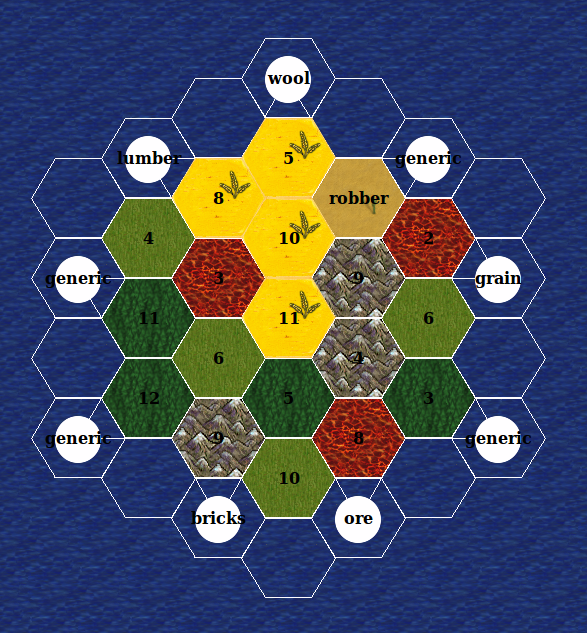
\includegraphics[width=\linewidth]{board.png}
  \end{center}
  \caption{Wygląd przykładowej planszy do gry z włączonymi stylami
    \emph{CSS}}
  \label{fig:board}
\end{figure}

\clearpage

\section{Implementacja klienta}

Początkowo do implementacji części klienckiej wykorzystana została
biblioteka \emph{jQuery}, wraz z \emph{jQuery UI}. Biblioteka
\emph{jQuery} została stworzona przez Johna Resiga w 2006
roku. Głównymi cechami \emph{jQuery} są: minimalizm i łatwa
rozszerzalność za pomocą ,,wtyczek''. Na bazie \emph{jQuery} powstała
również biblioteka \emph{jQuery UI}, która udostępnia podstawowe
elementy interfejsu użytkownika, takie jak: okna dialogowe,
kalendarze, itp. Podczas implementacji kodu klienta okazało się
jednak, że niewielka liczba funkcji bibliotecznych jest dość uciążliwa
i powoduje konieczność korzystania z zewnętrznych rozszerzeń. Pomimo
pozornie dużego wyboru dostępnych ,,wtyczek'', w wielu przypadkach
niezbędne jest wprowadzenie do nich własnych poprawek, a jakość ich
kodu pozostawia wiele do życzenia.

Inną ciekawą biblioteką \emph{JavaScript} jest \emph{Yahoo! User
  Interface Library}. Najważniejszym czynnikiem, który wpłynął na
decyzję o zmianie biblioteki na \emph{YUI} było wydanie wersji
\emph{3.0.0 beta 1}, dnia 24 czerwca 2009 roku. W porównaniu do
poprzednich wersji, biblioteka \emph{YUI3} została przeprojektowana i
w większości zaimplementowana od początku. Jej twórcy zapożyczyli
także najlepsze rozwiązania innych bibliotek, m.in. mechanizm
selektorów \emph{jQuery}. \emph{YUI3} oferuje bardzo bogaty zestaw
gotowych narzędzi, z których najważniejsze z punktu widzenia
tworzonego projektu to:

\begin{itemize}
\item ,,klasa''\footnote{w języku \emph{JavaScript} formalnie nie
    istnieje pojęcie klasy. W praktyce okazuje się jednak, że
    zastosowany mechanizm bezklasowy wykorzystywany jest podobny
    sposób do tradycyjnego} \texttt{Base} udostępniająca podstawowe
  mechanizmy znane z klasycznych języków obiektowych, takie jak:
  kontruktory i destruktory, atrybuty wraz z metodami dostępowymi
  (\texttt{get} i \texttt{set})
\item ,,klasa'' \texttt{Widget} będąca podstawą dla wszystkich
  tworzonych kontrolek
\item funkcje takie jak \texttt{augment}, \texttt{extend} i
  \texttt{aggregate}, ułatwiające dziedziczenie obiektów (ponowne
  wykorzystanie kodu)
\item najważniejsze funkcje ułatwiające pracę z kolekcjami,
  m.in. \texttt{map}, \texttt{reduce}, \texttt{find}
\end{itemize}

Należy zaznaczyć fakt, że biblioteka \emph{YUI3} znajduje się ciągle w
fazie intensywnego rozwoju -- niektóre jej elementy mogą ulec zmianie
w wersji \emph{3.0.0 GA} (ang. General Availability). Do czasu wydania
wersji \emph{GA}, nie jest zalecane wykorzystanie biblioteki w
środowiskach produkcyjnych. Konsekwencją wyboru \emph{YUI3} jest
również stosunkowo niewielka społeczność skupiona wokół biblioteki. Do
tej pory dostępne są jedynie bardzo nieliczne przykłady wykorzystania
\emph{YUI3} oraz jej rozszerzenia. Pomimo tych niedogodności
biblioteka ta jest warta uwagi, gdyż zbudowana została na bardzo
solidnych fundamentach. W niedalekiej przyszłości może ona okazać się
poważnym konkurentem dla dominujących dzisiaj rozwiązań, takich jak
\emph{jQuery}.

\subsection{Logika gry}
W przypadku tradycyjnych aplikacji internetowych, niepoprawne dane
wysyłane są do serwera, który zwraca w odpowiedzi błędy
walidacji. Zastosowanie tego mechanizmu wprowadziłoby do gry
niepotrzebne opóźnienia oraz stanowiłoby spore utrudnienie,
szczególnie dla początkujących graczy.

Dla sprawnego działania gry niezbędna jest możliwość stwierdzenia
poprawności generowanych zapytań, jeszcze przed wysłaniem ich do
serwera. W tym celu konieczne okazało się zaimplementowanie po stronie
klienta następujących ,,klas'':

\begin{itemize}
\item \texttt{Game} - przechowuje podstawowe informacje o stanie gry,
  listę graczy, aktualną ofertę oraz obiekt \texttt{Board}
\item \texttt{Player} - informacje i stan gracza
\item \texttt{Offer} - informacje o ofercie handlu złożonej przez
  jednego z graczy, wraz z listą odpowiedzi
\item \texttt{Board}, \texttt{Edge}, \texttt{Hex}, \texttt{Node} -
  informacje o planszy do gry, wszystkich jej sześciokątach,
  wierzchołkach i krawędziach
\end{itemize}

Wszystkie powyższe ,,klasy'' dziedziczą po ,,klasie'' \texttt{Base}. W
celu uniknięcia kolizji nazw, umieszczone zostały one w przestrzeni
nazw \texttt{Pioneers}. Po uruchomieniu skryptu (otworzeniu strony z
grą) pobierane są dane gry w formacie \emph{JSON}. Po sparsowaniu
danych przekazywane są one do konstruktora obiektu \texttt{Game},
który odpowiedzialny jest za utworzenie wszystkich powiązanych
obiektów. W trakcie trwania rozgrywki niezbędne jest aktualizowanie
danych dotyczących gry, poprzez metodę \texttt{setAttrs} obiektu
\texttt{Game}. Opisywane ,,klasy'' stanowią uproszczoną wersję klas
modeli, opisywanych w rozdziale \ref{sec:models}.

Oczywiście walidacja poszczególnych posunięć graczy nie może odbywać
się wyłącznie po stronie klienta. Serwer jest w dalszym ciągu
odpowiedzialny za ostateczne sprawdzenie poprawności działań graczy, w
celu uniemożliwienia nieprzepisowych zagrań, np. poprzez fałszowanie
treści zapytań.

\subsection{Elementy interfejsu graficznego}

,,Klasą'' bazową dla elementów interfejsu graficznego w bibliotece
\emph{YUI} jest ,,klasa'' \texttt{Widget}. W przeciwieństwie do
biblioteki \emph{jQuery UI}, wprowadzone zostały pewne konwencje
tworzenia kontrolek. Zastosowanie się do nich znakomicie upraszcza
implementację, a tworzony kod aplikacji staje się bardziej
spójny. Proces renderowania kontrolki podzielony jest na następujące
etapy:

\begin{enumerate}
\item \texttt{renderUI} - utworzenie wszystkich dodatkowych elementów
  strony (przycisków, etykiet, itp.)
\item \texttt{bindUI} - powiązanie zdarzeń interfejsu użytkownika z
  odpowiednimi funkcjami, odpowiedzialnymi za ich obsługę
\item \texttt{syncUI} - synchronizacja stanu wewnętrznego kontrolki z
  treścią znajdującą się na stronie
\end{enumerate}

Aby ułatwić nanoszenie stylów \emph{CSS} na kontrolki, składają się
one przynajmniej z dwóch, zagnieżdżonych znaczników
\texttt{<div>}. Pierwszy z nich, nazwany \emph{Bounding Box}, ułatwia
tworzenie efektów, takich jak zaokrąglone krawędzie i cienie. Drugi,
tzw. \emph{Content Box} obejmuje właściwą zawartość
kontrolki. Ujednolicone zostało także nazewnictwo klas, nadawanych
poszczególnym elementom składowym kontrolki. W celu uniknięcia kolizji
oznaczeń, nazwy klas elementów znajdujących się wewnątrz kontrolki
poprzedzone są odpowiednim prefiksem. Schemat zagnieżdżenia
znaczników, wraz z przykładowymi nazwami klas przedstawiony został na
\imref{fig:widget}.

\begin{figure}[ht]
  \begin{center}
    \includegraphics[width=\linewidth]{widget}
  \end{center}
  \caption{Schemat zagnieżdżenia znaczników \emph{HTML} kontrolki
    \texttt{Game} wraz z przykładowymi oznaczeniami klas}
  \label{fig:widget}
\end{figure}

Interfejs graficzny użytkownika składa się z zestawu niezależnych od
siebie kontrolek, komunikujących się ze sobą przeważnie za pomocą
zdarzeń. Z reguły kontrolki te przystosowane są do realizacji prostych
zadań, będąc częściami składowymi większych elementów. Najważniejszą
kontrolką jest \texttt{Game}, odpowiedzialna za utworzenie i obsługę
zdarzeń następujących obiektów:

\begin{itemize}
\item \texttt{GameStatus} - wyświetlanie informacji o stanie gry
\item \texttt{Players} - wyświetlanie listy graczy i ogólnych
  informacji o każdym z nich
\item \texttt{UserPlayer} - szczegółowe informacje o zalogowanym graczu
\item \texttt{Join} - dołączanie do rozgrywki
\item \texttt{Board} - plansza do gry
\item \texttt{AfterRoll} - kończenie tury
\item \texttt{BeforeRoll} - rzut kośćmi do gry
\item \texttt{Build} - budowanie osad, dróg i miast oraz kupowanie
  kart rozwoju
\item \texttt{Cards} - lista posiadanych kart
\item \texttt{Discard} - odrzucanie kart zasobów w fazie rozbójnika
\item \texttt{Exchange} - wymiana zasobów z bankiem
\item \texttt{Offer} - tworzenie ofert handlu
\item \texttt{OfferReceived} - wyświetlenie oferty utworzonej przez
  innego gracza z możliwością akceptacji lub odrzucenia
\item \texttt{OfferSent} - podgląd wysłanej oferty handlu i
  otrzymanych odpowiedzi
\end{itemize}

Obiekt \texttt{Game} odpowiedzialny jest także za komunikację z
serwerem.

\begin{itemize}
\item \texttt{YearOfPlenty} - używany w przypadku zagrania karty
  rozwoju ,,wynalazek''
\item \texttt{Monopoly} - używany w przypadku zagrania karty
  ,,monopol''
\end{itemize}

% TODO
% zawierają inne widgety (Game, Cards)
% korzystają z danych zawartych w poprzednich klasach
% wywołują eventy przechwytywane przez Game, który odpowiedzialny jest
% za komunikację z serwerem


\begin{figure}[ht]
  \begin{center}
    \begin{tabular}{cc}
      \subfloat[Rzut kością]{\label{fig:beforerollwidget}}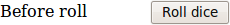
\includegraphics[scale=0.45]{beforerollwidget.png}
      &
      \subfloat[Kończenie tury]{\label{fig:afterrollwidget}}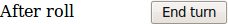
\includegraphics[scale=0.45]{afterrollwidget.png}
      \\[40pt]
      \subfloat[Budowa drogi, osady, miasta lub zakup karty rozwoju]{\label{fig:buildwidget}}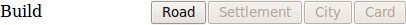
\includegraphics[scale=0.45]{buildwidget.png}
      &
      \subfloat[Lista posiadanych kart rozwoju]{\label{fig:cardswidget}}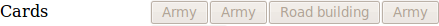
\includegraphics[scale=0.45]{cardswidget.png}
      \\[40pt]
      \subfloat[Odrzucanie nadmiarowych zasobów w fazie ,,rozbójnika'']{\label{fig:discardwidget}}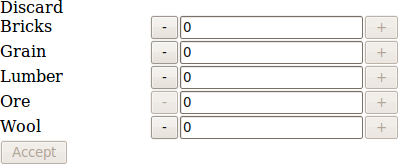
\includegraphics[scale=0.45]{discardwidget.png}
      &
      \subfloat[Tworzenie wymiany z bankiem]{\label{fig:exchangewidget}}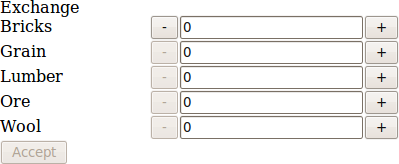
\includegraphics[scale=0.45]{exchangewidget.png}
      \\[40pt]
      \subfloat[Tworzenie oferty handlu]{\label{fig:offerwidget}}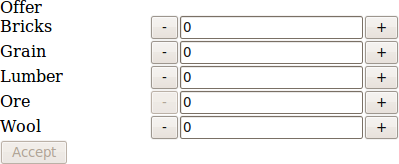
\includegraphics[scale=0.45]{offerwidget.png}
      &
      \subfloat[Dołączanie do rozgrywki]{\label{fig:joinwidget}}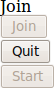
\includegraphics[scale=0.45]{joinwidget.png}
      \\[40pt]
      \subfloat[Podgląd otrzymanej oferty handlu]{\label{fig:offerreceivedwidget}}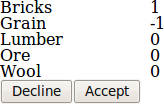
\includegraphics[scale=0.45]{offerreceivedwidget.png}
      &
      \subfloat[Podgląd utworzonej oferty handlu]{\label{fig:offersentwidget}}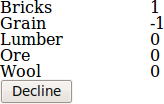
\includegraphics[scale=0.45]{offersentwidget.png}
      \\[40pt]
      \subfloat[Podgląd gracza]{\label{fig:userplayerwidget}}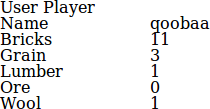
\includegraphics[scale=0.45]{userplayerwidget.png}
      &
      \subfloat[Lista pozostałych graczy]{\label{fig:playerswidget}}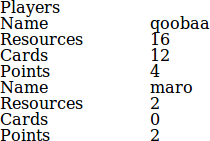
\includegraphics[scale=0.45]{playerswidget.png}
      \\[40pt]
      \subfloat[Podgląd stanu gry]{\label{fig:gamestatuswidget}}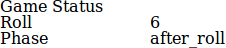
\includegraphics[scale=0.45]{gamestatuswidget.png}
      & \\
    \end{tabular}
  \end{center}
  \caption{Wygląd kontrolek}
  \label{fig:widgets}
\end{figure}

\subsection{Komunikacja z serwerem}

W związku z tym, że jednym z głównych założeń projektowych jest
możliwość dostosowania aplikacji do wymagań stawianych przez
urządzenia mobilne, komunikacja z serwerem została oparta o tradycyjny
\emph{Ajax} (\emph{HTTP Pull}). Opóźnienia wynikające z użycia tego
rozwiązania nie stanowią większego problemu w przypadku implementacji
gier turowych. Cykliczne pobieranie danych gry w kilkusekundowych
odstępach jest zupełnie wystarczające z punktu widzenia użytkownika,
nie wprowadza również nadmiernego obciążenia serwera gry.

Aby uniknąć problemów z niespójnością danych i konieczności
synchronizowania klientów, każdorazowo pobierane są kompletne dane o
rozgrywce, zawierające m.in.:

\begin{itemize}
\item informacje o grze - stan, fazę, numer aktualnego gracza,
  aktualny wynik rzutu kością, itp.
\item informacje o planszy, wszystkich jej sześciokątach,
  wierzchołkach i krawędziach
\item listę graczy, informacje o liczbie poszczególnych kart zasobów,
  jawnych punktów, liczbie posiadanych kart rozwoju
\item informacje o aktualnej ofercie handlowej oraz zagranej karcie
  rozwoju
\end{itemize}

Dodatkowo, jeżeli zalogowany użytkownik jest uczestnikiem rozgrywki,
wysyłane są również informacje o:

\begin{itemize}
\item numerze gracza należącego do użytkownika
\item poszczególnych kartach rozwoju, będących w jego posiadaniu
\end{itemize}

Jeśli zalogowany użytkownik nie jest uczestnikiem rozgrywki, otrzymuje
jedynie ogólne informacje o grze. W takim przypadku wyświetlany jest
tylko podstawowy interfejs graficzny, umożliwiający śledzenie
gry. Wydawać by się mogło, że przesyłanie informacji o liczbie
poszczególnych kart zasobów graczy jest sprzeczne z zasadami gry.
Zgodnie z zasadami, pozostali gracze mają dostęp jedynie do informacji
o liczbie wszystkich kart zasobów posiadanych przez danego gracza. Po
przeanalizowaniu tego problemu można dojść do wniosku, że jest on
analogiczny do zakrywania zagranych lew np. w grze w brydża. Jeżeli
nie mamy możliwości kontrolowania zachowania gracza (co ma miejsce w
przypadku gry na odległość), to może on notować wszystkie zagrane
karty. Możliwe jest również napisanie prostego skryptu, który będzie
automatyzował tę czynność, wyświetlając żądane informacje. Sytuacja
taka ma miejsce, ponieważ niemal wszystkie ,,przepływy'' surowców w
grze są jawne\footnote{oryginalne zasady gry nie precyzują tej kwestii
  w kilku przypadkach, mają one jednak znikomy wpływ na przebieg
  rozgrywki}. W celu zachowania zgodności z zasadami gry, wyświetlana
jest jedynie sumaryczna liczba kart zasobów poszczególnych
graczy. Jedyną prawdziwie ,,utajnioną'' informacją jest informacja o
rodzajach posiadanych przez graczy kart zasobów. W tym przypadku żadne
uproszczenia nie były możliwe, gdyż jest to bardzo istotny element
rozgrywki.

Mogłoby się wydawać, że zastosowany mechanizm komunikacji jest
nieoptymalny i powoduje niepotrzebny wzrost ilości przesyłanych
informacji. Danych tych jest w rzeczywistości dość niewiele, a
wykorzystanie formatu \emph{JSON} powoduje, że całkowity rozmiar
pobieranych danych nie przekracza kilku kilobajtów\footnote{większość
  danych przesyłanych pomiędzy przeglądarką a serwerem jest dodatkowo
  kompresowana przez serwer \emph{HTTP} (zwykle wykorzystywany jest
  \emph{gzip}). Jako, że dane w formacie \emph{JSON} zapisywane są
  zwykłym tekstem, zastosowanie nawet prostego algorytmu kompresji
  pozwala znacząco zmniejszyć ich objętość}.

Po wykonaniu dowolnego działania przez gracza, w tle wysyłane jest
żądanie \emph{HTTP}. Jeśli otrzymane żądanie jest poprawne,
odpowiedzią serwera jest przekierowanie do akcji \texttt{show}
kontrolera \texttt{GamesController} (a więc pobranie danych gry),
dzięki czemu gracz widzi niemal natychmiastowy rezultat swojego
działania. W przypadku pozostałych uczestników rozgrywki, rezultaty
widoczne są po dopiero kilku sekundach. Dopóki jednak pomiędzy
poszczególnymi pobraniami danych nie zostanie wywołana więcej niż
jedna akcja, pozostali gracze odnoszą wrażenie płynności gry. Takie
rozwiązanie znacząco poprawia komfort rozgrywki i znakomicie sprawdza
się w przypadku gier turowych, takich jak ,,Osadnicy z Catanu''.

\clearpage

\bibliographystyle{plain}
\bibliography{praca}

\end{document}
